\documentclass[12pt]{report}
\usepackage[italian]{babel}
\usepackage{enumitem}
\usepackage{comment}
\usepackage{graphicx} %per le immagini
\usepackage{textcomp} %per fare le frecce a destra
\usepackage{multicol,float} %per creare colonne
\usepackage[table,xcdraw]{xcolor} %colore tabella
\usepackage{listings} %per mettere il codice
\usepackage{color} % per i colori
\usepackage{array}




%java format
\definecolor{dkgreen}{rgb}{0,0.6,0}
\definecolor{gray}{rgb}{0.5,0.5,0.5}
\definecolor{mauve}{rgb}{0.58,0,0.82}
\lstset{frame=tb,
	language=Java,
	aboveskip=3mm,
	belowskip=3mm,
	showstringspaces=false,
	columns=flexible,
	basicstyle={\small\ttfamily},
	numbers=none,
	numberstyle=\tiny\color{gray},
	keywordstyle=\color{blue},
	commentstyle=\color{dkgreen},
	stringstyle=\color{mauve},
	breaklines=true,
	breakatwhitespace=true,
	morecomment=[s][\color{gray}]{@}{\ },
	tabsize=3
}


%json style
\colorlet{punct}{red!60!black}
\definecolor{background}{HTML}{EEEEEE}
\definecolor{delim}{RGB}{20,105,176}
\colorlet{numb}{magenta!60!black}
\lstdefinelanguage{json}{
	basicstyle=\normalfont\ttfamily,
	literate=
	{:}{{{\color{punct}{:}}}}{1}
	{,}{{{\color{punct}{,}}}}{1}
	{\{}{{{\color{delim}{\{}}}}{1}
	{\}}{{{\color{delim}{\}}}}}{1}
	{[}{{{\color{delim}{[}}}}{1}
	{]}{{{\color{delim}{]}}}}{1},
}




\usepackage{uniudtesi} %prima pagina tesi formato uniud
\date{21 Novembre 2019} %se ommesso imposta la data odierna nel formato dd Mese anno in inglese
\author{Alberto Caliman}
\titolo{Progettazione e sviluppo di \\un'applicazione Android per \\la gestione degli orari di lavoro}
\laureando{Alberto Caliman}
% \laureando{Giovanni Tesista}
\annoaccademico{2018-2019}
% \facolta{Scienze Matematiche, Fisiche e Naturali} % (default)
%  \corsodilaurea{Informatica} % per la laurea vecchio ordinamento
\corsodilaureatriennalein{Informatica}
% \corsodilaureaspecialisticain{Informatica}
% \corsodilaureamagistralein{Matematica}
\relatore[Dott.]{Stefano burigat}
%  \relatoreDue[Prof.]{Secondo relatore}
% \correlatore{Talaltro dei Tali}
% \correlatoreDue{Secondo Correlatore}
%\dedica{A Me stesso} % (facoltativo)
\usepackage[pdfa]{hyperref} %libreria link
\begin{document}
\maketitle %mostra il titolo
\newpage\null\thispagestyle{empty}\newpage
\tableofcontents %indice
	%\newpage crea una nuova pagina
\newpage

  \chapter*{Introduzione}
  La presente tesi descrive il processo di progettazione e sviluppo di un'applicazione mobile Android svolto durante l'attività di tirocinio presso l'azienda Sinesy Srl\cite{Sinesy}.\\
  L'applicazione nasce con l'idea di realizzare un prodotto veloce, intuitivo e semplice per permettere ai dipendenti dell'azienda di gestire le presenze e gli orari di lavoro. Essa affianca un sito web esistente, il quale permette di svolgere tali attività in modo più complesso e non chiaro a utenti non tecnici.
 Il lavoro svolto ha previsto una fase di progettazione in cui sono stati studiati i requisiti funzionali, non funzionali e quelli di dominio. In seguito si è svolta un'attività di studio delle interfacce in modo da rendere il prodotto finale di facile utilizzo per gli utenti. Attraverso un brainstorming e dei prototipi si sono studiati i task principali che i dipendenti svolgono abitualmente, in modo da ottimizzarli al meglio e renderli più intuitivi. Alla fine del processo di design sono stati realizzati dei prototipi ad alto livello i quali, hanno permesso agli sviluppatori, di realizzare le interfacce utente. Il team del progetto al quale ho collaborato, mi ha permesso di comprendere le varie architetture mobile studiandone vantaggi e svantaggi per poi infine implementare quella che meglio si adattava all'applicazione. L'utilizzo del linguaggio di programmazione Java e dell'ambiente Android Studio 3.0\cite{Android} hanno permesso di implementare il software finale e i relativi test strumentali per verificare il corretto funzionamento dell'applicazione realizzata.

%%\newpage\null\thispagestyle{empty}\newpage
\chapter{Analisi dei requisiti}
In questo capitolo viene descritta la fase di scoperta ed elicitazione dei requisiti del sistema. Questa fase è particolarmente significativa per lo sviluppo dell'applicazione finale in quanto costituisce la base per le successive attività: progettazione, implementazione e testing. Dei requisiti non definiti in modo chiaro, univoco, coerente e completo possono portare al fallimento dell'intero progetto. I requisiti si suddividono in tre categorie: \textit{funzionali, non funzionali e di dominio}.
\begin{enumerate}[]
\item I requisiti funzionali descrivono cosa deve fare il sistema, generalmente
in termini di relazioni fra dati di ingresso e dati di uscita, oppure fra stimoli (dall’ambiente al sistema) e risposte del sistema. Questi sono
generalmente esprimibili in modo formale.

\item I requisiti non funzionali esprimono dei vincoli o delle caratteristiche di
qualità. Quest'ultime sono più difficili da esprimere in modo formale, in
particolare è difficile esprimerle in modo quantitativo. Le principali caratteristiche di qualità
 si suddividono in due famiglie. I \textit{parametri esterni} rappresentano la qualità del software così com'è percepita dagli utenti finali e includono: correttezza,  affidabilità, robustezza, usabilità. \textit{Parametri interni} si riferiscono alla qualità del software così com'è percepita dagli sviluppatori e includono verificabilità, riusabilità, manutenibilità e modularità.
\item I requisiti di dominio esprimono le caratteristiche che il sistema deve soddisfare in un determinato dominio di utilizzo, e provengono direttamente dal dominio applicativo. Se questi ultimi non vengono soddisfatti, il sistema diventa inusabile e solitamente ciò accade quando non vengono ben compresi o non sono sufficientemente chiari.
\end{enumerate}
È quindi di fondamentale importanza specificare al meglio i requisiti raccolti in modo che siano chiari, ben documentati, tracciabili e misurabili.%\\ In questa fase è stato coinvolto il team di sviluppo e dei dipendenti dell'azienda, questi ultimi hanno espresso quali secondo loro dovevano essere delle funzionalità importanti da realizzare.
\section{Definizione del problema}
I dipendenti dell'azienda, utilizzano un sito web datato per inserire gli orari di lavoro e le commesse alle quali hanno lavorato. Gli si vuole offrire un'applicazione mobile moderna e intuitiva, che gli permetta di gestire i propri orari di lavoro in qualsiasi momento, eseguendo il minimo numero di operazioni per inserire i dati. Inoltre si vuole rendere l'operazione di inserimento delle ore di lavoro e delle commesse più semplice, intuitiva e veloce.
\section{Utenti coinvolti}
L'applicazione coinvolge diverse figure all'interno dell'azienda (stakeholder), che operano in modo coordinato per raggiungere un obiettivo comune. Gli stakeholder rappresentano l'insieme delle persone che vengono influenzate dal sistema finale.\\
Gli stakeholder \textit{interni} sono parte attiva dell'azienda e influenzano direttamente il prodotto finale. Essi comprendono:
\begin{itemize}
	\item CEO (Chief Executive Officer) e CFO (Chief Founder Officer): sono i fondatori di Sinesy
	\item Sviluppatori front-end, back-end: operano direttamente nello sviluppo dell'applicazione influenzandone le modalità d'uso
	\item Grafici e designer: operano nelle interfacce e nella definizione dell'esperienza utente
	\item CMO (Chief Marketing Officer): adatta il prodotto in modo da renderlo vendibile e fruibile ai nuovi clienti e comunica le novità tramite l'utilizzo di social media e articoli
\end{itemize}
Gli stakeholder \textit{esterni} influenzano indirettamente il sistema, e sono rappresentati da:
\begin{itemize}
	\item Responsabili dell'ufficio stipendi: si occupano di calcolare lo stipendio secondo i dati inseriti dai dipendenti
	\item Fornitori: sono le aziende esterne che offrono le infrastrutture su cui si basa l'applicazione
\end{itemize}

\section{Elicitazione e scoperta dei requisiti}
%Durante la scoperta dei requisiti, gli utenti hanno emerso l'importanza di inserire tramite l'applicazione i tre elementi di seguito elencati.%
Esaminando il sito web presente sono emerse differenti caratteristiche fondamentali, che hanno influenzato lo sviluppo dell'applicazione finale. Il sito web permette all'utente di inserire tre elementi fondamentali per l'azienda.
\begin{enumerate}
	\item \textit{La timbratura} è caratterizzata da due coppie di valori \textit{[ingresso mattina, uscita mattina]} e \textit{[ingresso pomeriggio, uscita pomeriggio]}. L’intervallo del secondo elemento della coppia deve essere strettamente maggior di quello del primo elemento. Il dominio di utilizzo porta alla definizione del concetto di \textit{ore presenza} il quale indica le ore in cui un dipendente è presente fisicamente all’interno dell’azienda. Inoltre si definiscono le \textit{ore lavorate} cioè quelle in cui il dipendente è effettivamente impiegato in un’attività (commessa). La relazione tra le due è la seguente: $oreLavorate \leq orePresenza$.\\
	Ogni dipendente ha un turno di lavoro che deve coincidere con le ore timbrate. Questo vincolo può essere violato per diversi motivi: assenze e/o straordinari, i quali si suddividono in: segnalati, vengono svolti al mattino, ed extra effettuati alla sera. Un dipendente che svolge degli straordinari, può decidere di utilizzare il tempo accumulato lavorando un tempo inferiore a quello previsto dal suo turno giornaliero, oppure può richiedere il pagamento delle ore svolte in eccesso. In questo caso è tenuto a richiederle espressamente specificando gli straordinari richiesti i quali devono soddisfare il seguente vincolo: $0\leq  straordinaririchiesti \leq segnalati+extra$.
	\textit{Il recupero ore} è un'altra definizione che viene introdotta dal dominio di utilizzo. Il dipendente può esprimere la volontà di fermarsi più tempo in azienda per recuperare eventuale tempo perso durante la giornata, così da svolgere il numero di ore minimo previsto dal suo turno di lavoro.
	\item \textit{Le commesse} rappresentano quali lavori devono essere svolti all'interno dell'azienda. Ogni commessa è associata ad uno e un solo cliente ed è collegata ad una persona fisica che può essere un project manager, sviluppatore, designer, ecc.. la quale avrà il compito di eseguire delle operazioni che rappresentano le attività da svolgere. Ogni dipendente che svolge delle operazioni per una determinata commessa, è tenuto a specificare il tempo in cui è stato impegnato in una determinata operazione.
	\item \textit{Le trasferte} sono caratterizzate da un insieme di valori: alloggio, pranzo, cena, note, km percorsi e tipologia di auto. Questi attributi devono essere inseriti da chi svolge una trasferta in un determinato giorno, in modo tale da permettere a fine mese di ottenere il rimborso delle spese effettuate.
\end{enumerate}
Questi elementi sono il punto centrale dell'applicazione in quanto ogni dipendente dovrà inserire una timbratura e una o più commesse al giorno.\\Il tempo impiegato per definire e comprendere i vincoli e le relazioni che caratterizzano i tre elementi è stato di notevole rilievo, poichè un errore di comprensione avrebbe portato all'inserimento di dati non validi e quindi all'errato calcolo dello stipendio, creando dei danni economici all'azienda.
\section{Raccolta dei requisiti di sistema}
I requisiti sono stati raccolti tramite il brainstorming. Questa tecnica è utilizzata nelle riunioni di gruppo per generare idee su un determinato argomento o prodotto. Ad ogni persona del gruppo è richiesto di suggerire più idee possibili. % Nessuna idea è inizialmente respinta durante la sessione di storming.
Alla fine del processo di raccolta, le idee vengono discusse dal gruppo, valutate e selezionate per poi raggrupparle in classi. Nello sviluppo dell'applicazione la fase di brainstorming ha coinvolto 15 dipendenti (tecnici e non), il loro contributo ha permesso di evidenziare le principali proprietà che il sistema finale doveva offrire. Di seguito viene presentato un elenco che riporta le attività principali svolte dai dipendenti.
\begin{enumerate}
	\item (per tutti) Quando un dipendente arriva o esce dall'azienda, striscia il proprio badge nel timbratore inserendo così nel sistema l'orario di ingresso o uscita.
	\item (per tutti) Ogni giorno i dipendenti devono inserire le commesse alle quali hanno lavorato e per quanto tempo.
	\item (a volte) Quando un dipendente non arriva in orario, deve specificare tramite un giustificativo il proprio ritardo.
	\item (a volte) Un dipendente che si ferma più del tempo previsto dal suo orario contrattuale, ha svolto degli straordinari e deve specificare il motivo per il quale sono stati eseguiti.
	\item(per alcuni dipendenti, circa 10)
	Alcuni dipendenti come: PM, CFO, CFE, ecc..non sono tenuti a timbrare con il badge, in quanto il loro orario di lavoro è flessibile, ma devono comunque inserire le ore lavorate manualmente.
	\item (1 volta al mese, tutti i mesi per tutti) Ogni dipendente alla fine di un mese è obbligato a far coincidere in ogni giorno, le ore timbrate con le ore delle commesse inserite considerando così un giorno \textit{chiuso} e quindi non più modificabile.
	\item (1 volta al mese, tutti i mesi per circa metà dipendenti) I dipendenti che eseguono delle trasferte sono tenuti a inserire le spese effettuate.
	\item (1 volta al mese, tutti i mesi per i supervisori) Un dipendente che è supervisore di altri è tenuto, all'inizio di ogni mese a controllare il calendario dei dipendenti che gli afferiscono, verificando che le ore lavorate coincidano con le ore delle commesse inserite. Se tutto è conforme approverà i giorni del mese.
	\item (1 volta al mese, tutti i mesi per i supervisori) Un dipendente che è anche supervisore di altri può decidere di stampare ed esportare alcuni giorni del calendario del suo sottoposto.
	\item (a volte) Un dipendente che per motivi di salute, familiari o ferie non è presente a lavoro, è tenuto a specificare il motivo della sua assenza, tramite l'applicazione.

\end{enumerate}
\section{Flussi di iterazione}
I \textit{Data Flow Diagram}\cite{dfd} (DFD) utilizzano una notazione grafica per la descrizione del flusso di informazioni all'interno di un sistema. Queste notazioni, a partire da una fonte, passano per strumenti di memorizzazione ed elaborazione fino a produrre un determinato output.\\ La notazione prevede che le ellissi rappresentino dei processi, che trasformano i dati di ingresso in quelli di uscita, mentre i rettangoli rappresentano gli archivi che svolgono l'attività di memorizzare le informazioni. Le frecce rappresentano i dati che vengono associati a dei flussi, descritti utilizzando delle etichette.
Le funzionalità dei dfd permettono di descrivere un flusso di iterazione con diversi livelli, ognuno dei quali aggiunge maggiori dettagli al precedente. Il livello 0 è quello che possiede un minor livello di dettaglio, il sistema viene rappresentato con un singolo nodo e i flussi di dati scambiati con le entità esterne. Scendendo nei vari livelli, i processi vengono scomposti aggiungendo sempre maggiori dettagli. \\
In questo caso, il dfd di livello 1 usato per rappresentare il flusso di timbratura è il seguente:
\begin{figure}[!h]
	\centering
	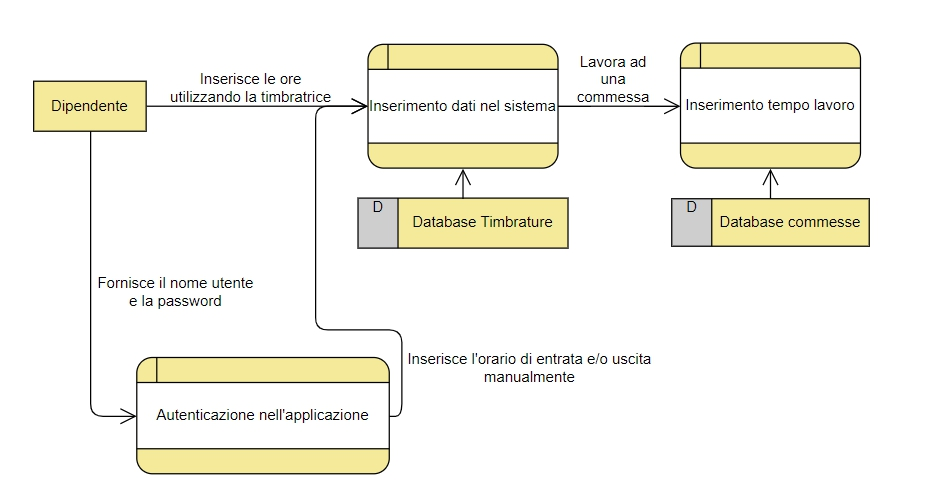
\includegraphics[width=1\linewidth]{immagini/dfd}
	\caption{}
	\label{fig:dfd}
\end{figure}
\\
Il dipendente utilizza una timbratrice di rete per segnalare le proprie entrate o uscite. Un processo nel server si occupa di raccogliere ogni 2 ore i dati dal timbratore e inserirli nel database. Successivamente l'utente potrà visualizzare i dati con le proprie ore nell'applicazione, dove eventualmente potrà aggiungere le informazioni di ritardi o straordinari. Un dipendente che non riesce ad utilizzare il timbratore, tramite l'applicazione può eseguire una timbratura manuale specificando l'orario di ingresso e uscita.

\section{Documento dei requisiti}
Il documento dei requisiti software rappresenta ciò che deve essere implementato dagli sviluppatori. Contiene sia requisiti utente che di sistema. Il documento coinvolge un numero di utenti vario, dai maggiori dirigenti dell'organizzazione, che avranno il ruolo di vendere e finanziare il prodotto finale, agli ingegneri responsabili dello sviluppo del software. Il documento dei requisiti viene specificato tramite degli standard definiti dal IEEE. Il più utilizzato è IEEE/ANSI 830-1998\cite{IEEEANSI830} il quale è composto da: un'introduzione che descrive il motivo per cui il sistema è necessario e come si adatta agli obiettivi commerciali, un glossario che definisce i termini tecnici utilizzati, il modello del sistema che definisce le varie componenti e come esse interagiscono tra loro. Contiene inoltre: la definizione dei requisiti funzionali e non, le evoluzioni che il sistema avrà nel tempo, come esso si evolverà e quali potranno essere le future modifiche, infine una specifica e dettagliata definizione dei requisiti.\\
Il documento dei requisiti è importante nello sviluppo di applicazioni di media grande complessità, perchè permette di comunicare e definire al meglio quali sono le esigenze e problemi dei clienti.\\
Nel progetto i requisiti proposti nella fase di analisi sono stati definiti in modo chiaro ed esaustivo e raggruppati tra loro, in modo che fossero coerenti e correlati.
Di seguito viene riportato un elenco dei principali requisiti raccolti.

\begin{figure}[h]
	\hspace*{-2,6cm}
	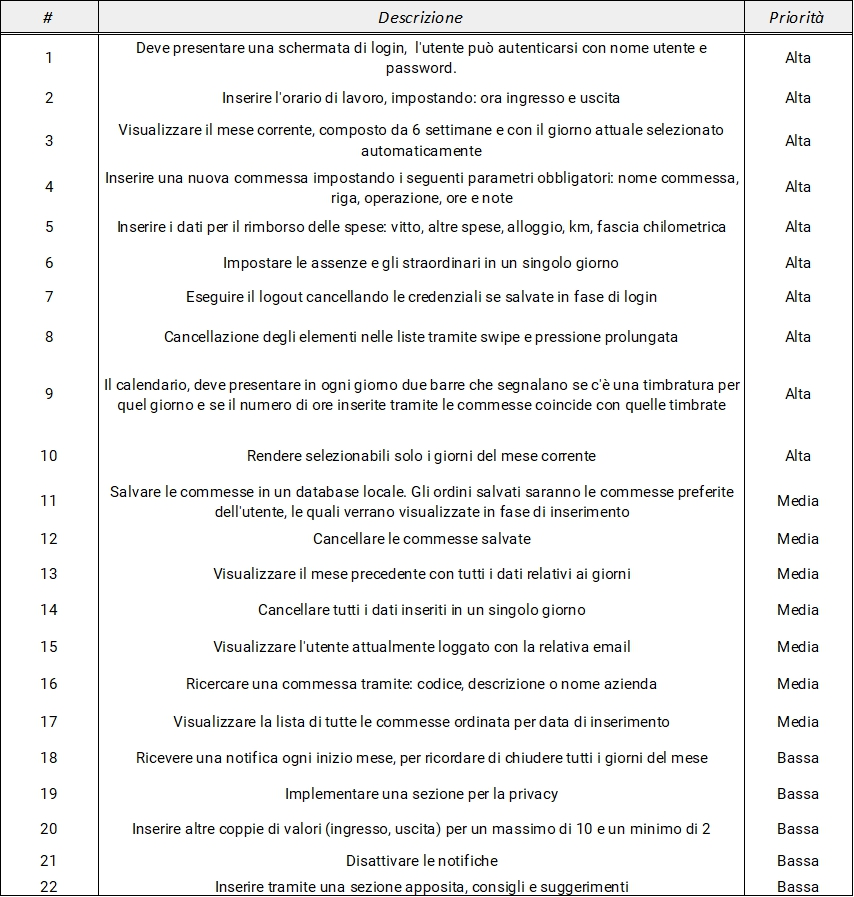
\includegraphics[width=1.3\linewidth]{immagini/tabella_requisiti}
\end{figure}
%\begin{table}
	\caption{Tabella requisiti}
	\begin{tabular}{||l||l|l|}
		\hline
		\# & Descrizione & Priorità \\ \hline
		1 & Deve presentare una schermata di login,  l'utente può autenticarsi con nome utente e password. & Alta \\ \hline
		2 & Inserire l'orario di lavoro, impostando: ora ingresso e uscita & Alta \\ \hline
		3 & Visualizzare il mese corrente, composto da 6 settimana e con il giorno attuale selezionato automaticamente & Alta \\ \hline
		4 & Inserire una nuova commessa impostando i seguenti parametri obbligatori: nome commessa, riga, operazione, ore e note & Alta \\ \hline
		5 & Inserire i dati per il rimborso delle spese: vitto, altre spese, alloggio, km, fascia chilometrica & Alta \\ \hline
		6 & Impostare le assenze e gli straordinari in un singolo giorno & Alta \\ \hline
		7 & Eseguire il logout cancellando le credenziali se salvate in fase di login & Alta \\ \hline
		8 & Cancellazione degli elementi nelle liste tramite swipe e pressione prolungata & Alta \\ \hline
		9 & Il calendario, deve presentare in ogni giorno due barre che segnalano se c'è una timbratura per quel giorno e se il numero di ore inserite tramite le commesse coincide con quelle timbrate & Alta \\ \hline
		10 & Visualizzare sei settimane nel calendario e rendere selezionabili solo i giorni del mese corrente & Alta \\ \hline
		11 & Salvare le commesse in un database locale. Gli ordini salvati saranno le commesse preferite dell'utente, le quali verrano visualizzate in fase di inserimento & Media \\ \hline
		12 & Cancellare le commesse salvate & Media \\ \hline
		13 & Visualizzare il mese precedente con tutti i dati relativi ai giorni & Media \\ \hline
		14 & Cancellare tutti i dati inseriti in un singolo giorno & Media \\ \hline
		15 & Visualizzare l'utente attualmente loggato con la relativa email & Media \\ \hline
		16 & Ricercare una commessa tramite: codice, descrizione o nome azienda & Media \\ \hline
		17 & Visualizzare la lista di tutte le commesse ordinata per data di inserimento & Media \\ \hline
		18 & Ricevere una notifica ogni inizio mese che ricorda di chiudere tutti i giorni del mese & Bassa \\ \hline
		19 & Sezione privacy & Bassa \\ \hline
		20 & Inserire altre coppie di valori (ingresso, uscita) per un massimo di 10 e un minimo di 2 & Bassa \\ \hline
		21 & Disattivare le notifiche & Bassa \\ \hline
		22 & Inserire tramite una sezione apposita, consigli e suggerimenti & Bassa \\ \hline
	\end{tabular}
\end{table}

\chapter{Design}
Oggi il numero di utenti che interagisce con le interfacce grafiche è in continuo aumento. Studiare come l'utente utilizza l'applicazione permette a designer e sviluppatori di realizzare interfacce semplici e intuitive, permettendo all'utente di eseguire le operazioni in modo più veloce e commettendo un minor numero di errori. Durante la realizzazione delle interfacce è importante valutare attentamente caratteristiche come la \textit{User Experience Design UX} cioè l'insieme dei processi che hanno lo scopo di accrescere la soddisfazione dell’utente, migliorando l’usabilità di una pagina web o applicazione, la sua facilità di utilizzo, l’intuitività e l’interazione. Lo scopo finale è quello di migliorare l'esperienza utente, fornendogli ciò che desidera nel miglior modo possibile. Una buona UX viene raggiunta non solo attraverso il giusto accostamento di forme e colori, ma anche tramite l'ideazione di interfacce che rendano la navigazione fluida. Una definizione formale dell’esperienza utente è pubblicata nella normativa ISO 9241-210\cite{ISO9241210} e di seguito riportata.
\begin{center}
	\textit{A person's perceptions and responses that result from the use or anticipated use of a product, system or service.}
\end{center}
La seconda caratteristica da valutare quando si realizzano delle interfacce grafiche è la \textit{User Interface Design UI}. Lo scopo di tale processo è di guidare l'utente in modo chiaro e intuitivo all'interno dell'applicazione. Per raggiungere una buona UI,
è importante evidenziare in modo chiaro quali siano gli obiettivi finali che gli utenti dovranno raggiungere tramite l'utilizzo dell'applicazione. I fattori che hanno un impatto tangibile sulla UI sono: design delle interfacce, velocità di utilizzo, coerenza visiva e convenzioni. Quest'ultime aiutano l'utente a ritrovarsi in un ambiente familiare, in quanto conosce già il funzionamento di alcuni componenti utilizzati di frequente dalle applicazioni in commercio. Anche per l'UI è stata pubblicata una definizione formale nella normativa ISO 9241\cite{ISO9241} e di seguito riportata.
	\begin{center}
	\textit{The extent to which a product can be used by specified users to achieve specified goals with effectiveness, efficiency and satisfaction in a specified context of use.}
\end{center}
Uno studio di design ben fatto porta alla realizzazione di un insieme di schermate che appaiono chiare, gradevoli e con una navigazione semplice e coinvolgente, permettendo all'utente di raggiungere velocemente e in modo fluido l'obiettivo finale. %In Questa fase insieme al reparto di grafica mi sono occupato di studiare le diverse interfacce proposte, svolgere i test sugli utenti e infine validare le schermate per poi implementarle nell'applicazione finale.



\section{Prototyping}
La fase di progettazione del design prevede inizialmente la realizzazione di prototipi a basso livello.
Lo scopo principale di tale strumento è quello di esplorare velocemente e in modo economico quali sono le idee principali per le differenti finestre che verranno successivamente implementate. La tecnica più comune per creare dei prototipi a bassa fedeltà è lo sketching. Tramite dei post-it vengono disegnate le idee iniziali delle varie schermate. Successivamente mediante raffinamenti successivi, si modifica il design dei prototipi iniziali rendendoli più dettagliati. Ad esempio vengono aggiunti: font, colori, dimensione del testo e immagini. Alla fine i prototipi raggiungono una definizione elevata diventando così dei \textit{prototipi ad alta fedeltà} che verranno utilizzati dagli sviluppatori come modelli per realizzare le schermate e dal team di vendita per promuovere il prodotto. Nella realizzazione dell'applicazione il team di design si è occupato di realizzare i prototipi ad alto livello, applicando le euristiche di UI e UX dei dispositivi mobile Android. Successivamente sono stati definiti font, colori e componenti seguendo la coerenza visiva e la documentazione ufficiale di Android\cite{Material}, che definisce alcune buone regole per la realizzazione di interfacce chiare e pulite. \\
%In questa fase insieme al reparto della grafica sono state definite diverse schermate che hanno portato alla realizzazione di prototipi ad alto livello.
%\underline{potrei mettere un esempio delle regole nel caso volessi allungarla}
\newpage
\begin{figure}[h!]
	\centering
	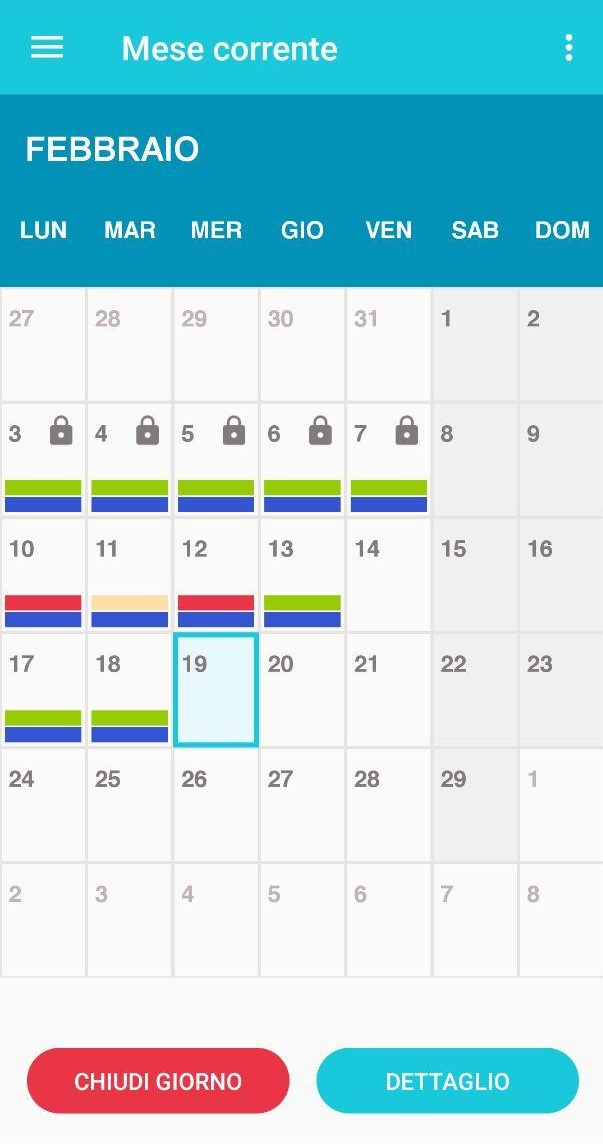
\includegraphics[width=0.35\linewidth]{immagini/home}
	\caption{}
\end{figure}
La schermata principale, sopra riportata, rappresenta il prototipo ad alto livello finale. É composta da un calendario che rappresenta il mese corrente e selezionato in blu, il giorno attuale. L'utente tramite un click può decidere di selezionare altri giorni del mese corrente. \\Le specifiche richiedono che nel calendario siano sempre visibili sei settimane. Per questo vengono inseriti a inizio e fine mese i giorni del mese precedente e successivo, tuttavia questi non sono selezionabili dall'utente. Lo sfondo del giorno cambia in base alla tipologia: nei giorni feriali o festivi è di un grigio più scuro mentre nei giorni lavorativi di uno più chiaro, in questo modo l'utente potrà distinguere più velocemente in quali giorni dovrà lavorare. Ogni giorno contiene al suo interno due indicatori: quello superiore indica che sono state inserite una o più commesse. Se di colore verde, le ore lavorate coincidono con quelle timbrate, se rosso, non c'è una corrispondenza tra ore lavorate e inserite, infine giallo se il numero di ore lavorate è maggiore rispetto alle ore standard lavorative di quella giornata. L'indicatore inferiore indica se è presente o meno una timbratura. Tramite il pulsante \textit{chiudi giorno} è possibile eseguire un'operazione (chiusura, approvazione e invio) su un singolo giorno, questo bottone è dinamico e in base allo stato del giorno l'operazione eseguibile sarà diversa. Il bottone \textit{dettaglio} permette di navigare nelle successive schermate, visualizzare e modificare i parametri del giorno selezionato.

\begin{multicols}{2}
 \begin{figure}[H]
	\centering
	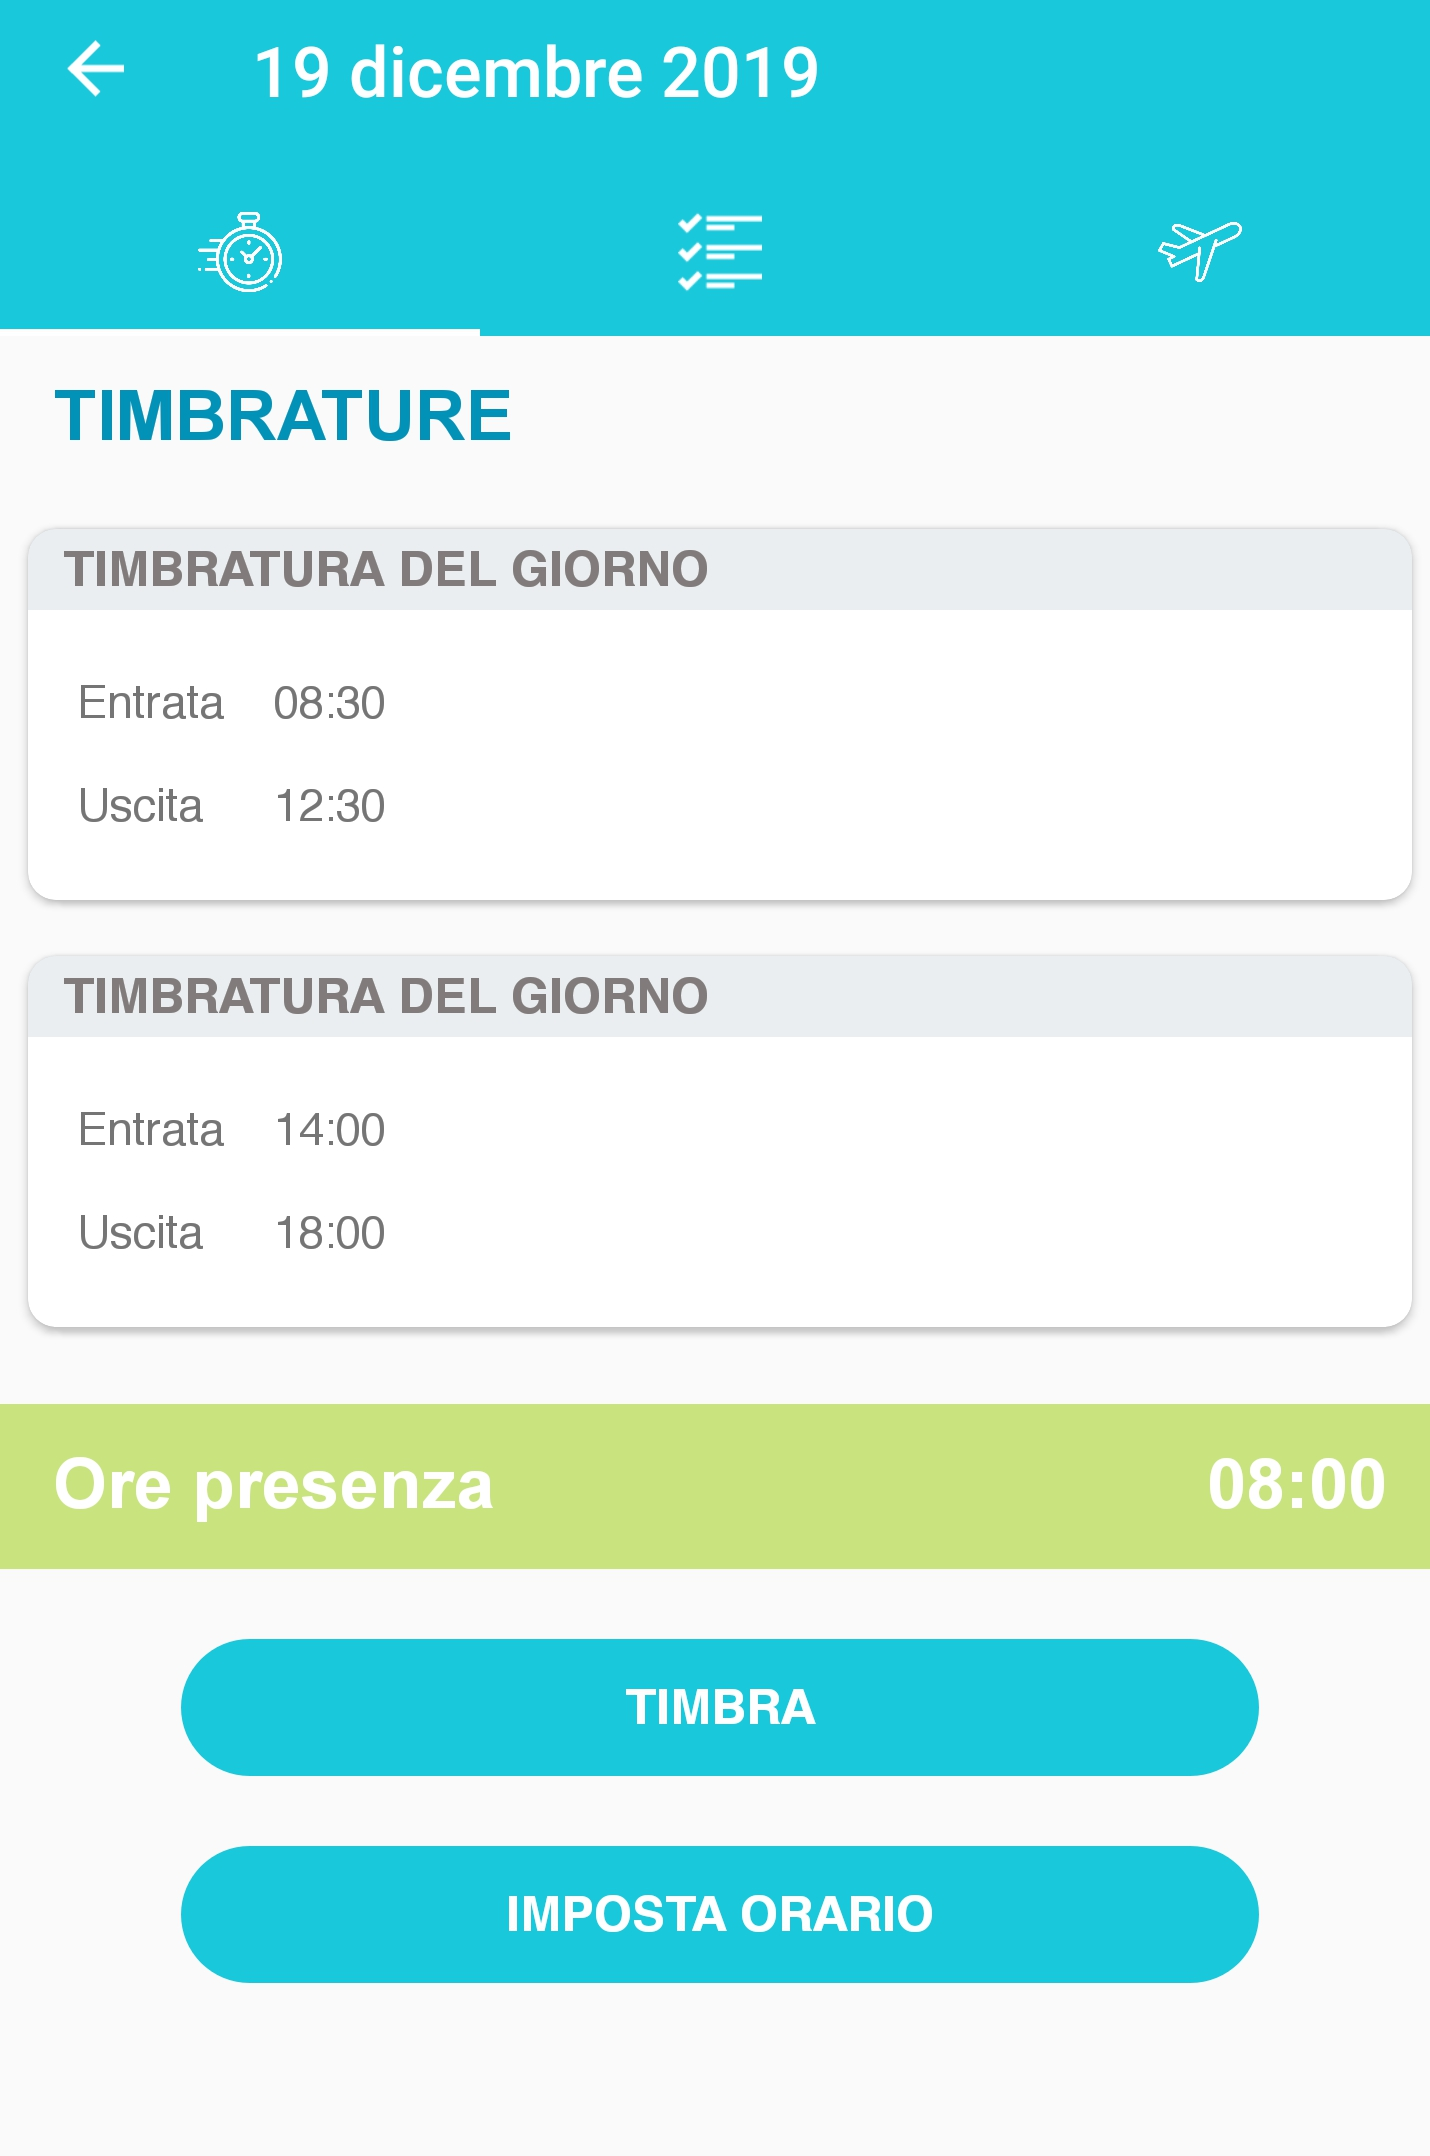
\includegraphics[width=0.8\linewidth]{immagini/timbrature}
	\caption{}
	\label{fig:timbrature}
\end{figure}
\begin{figure}[H]
	\centering
	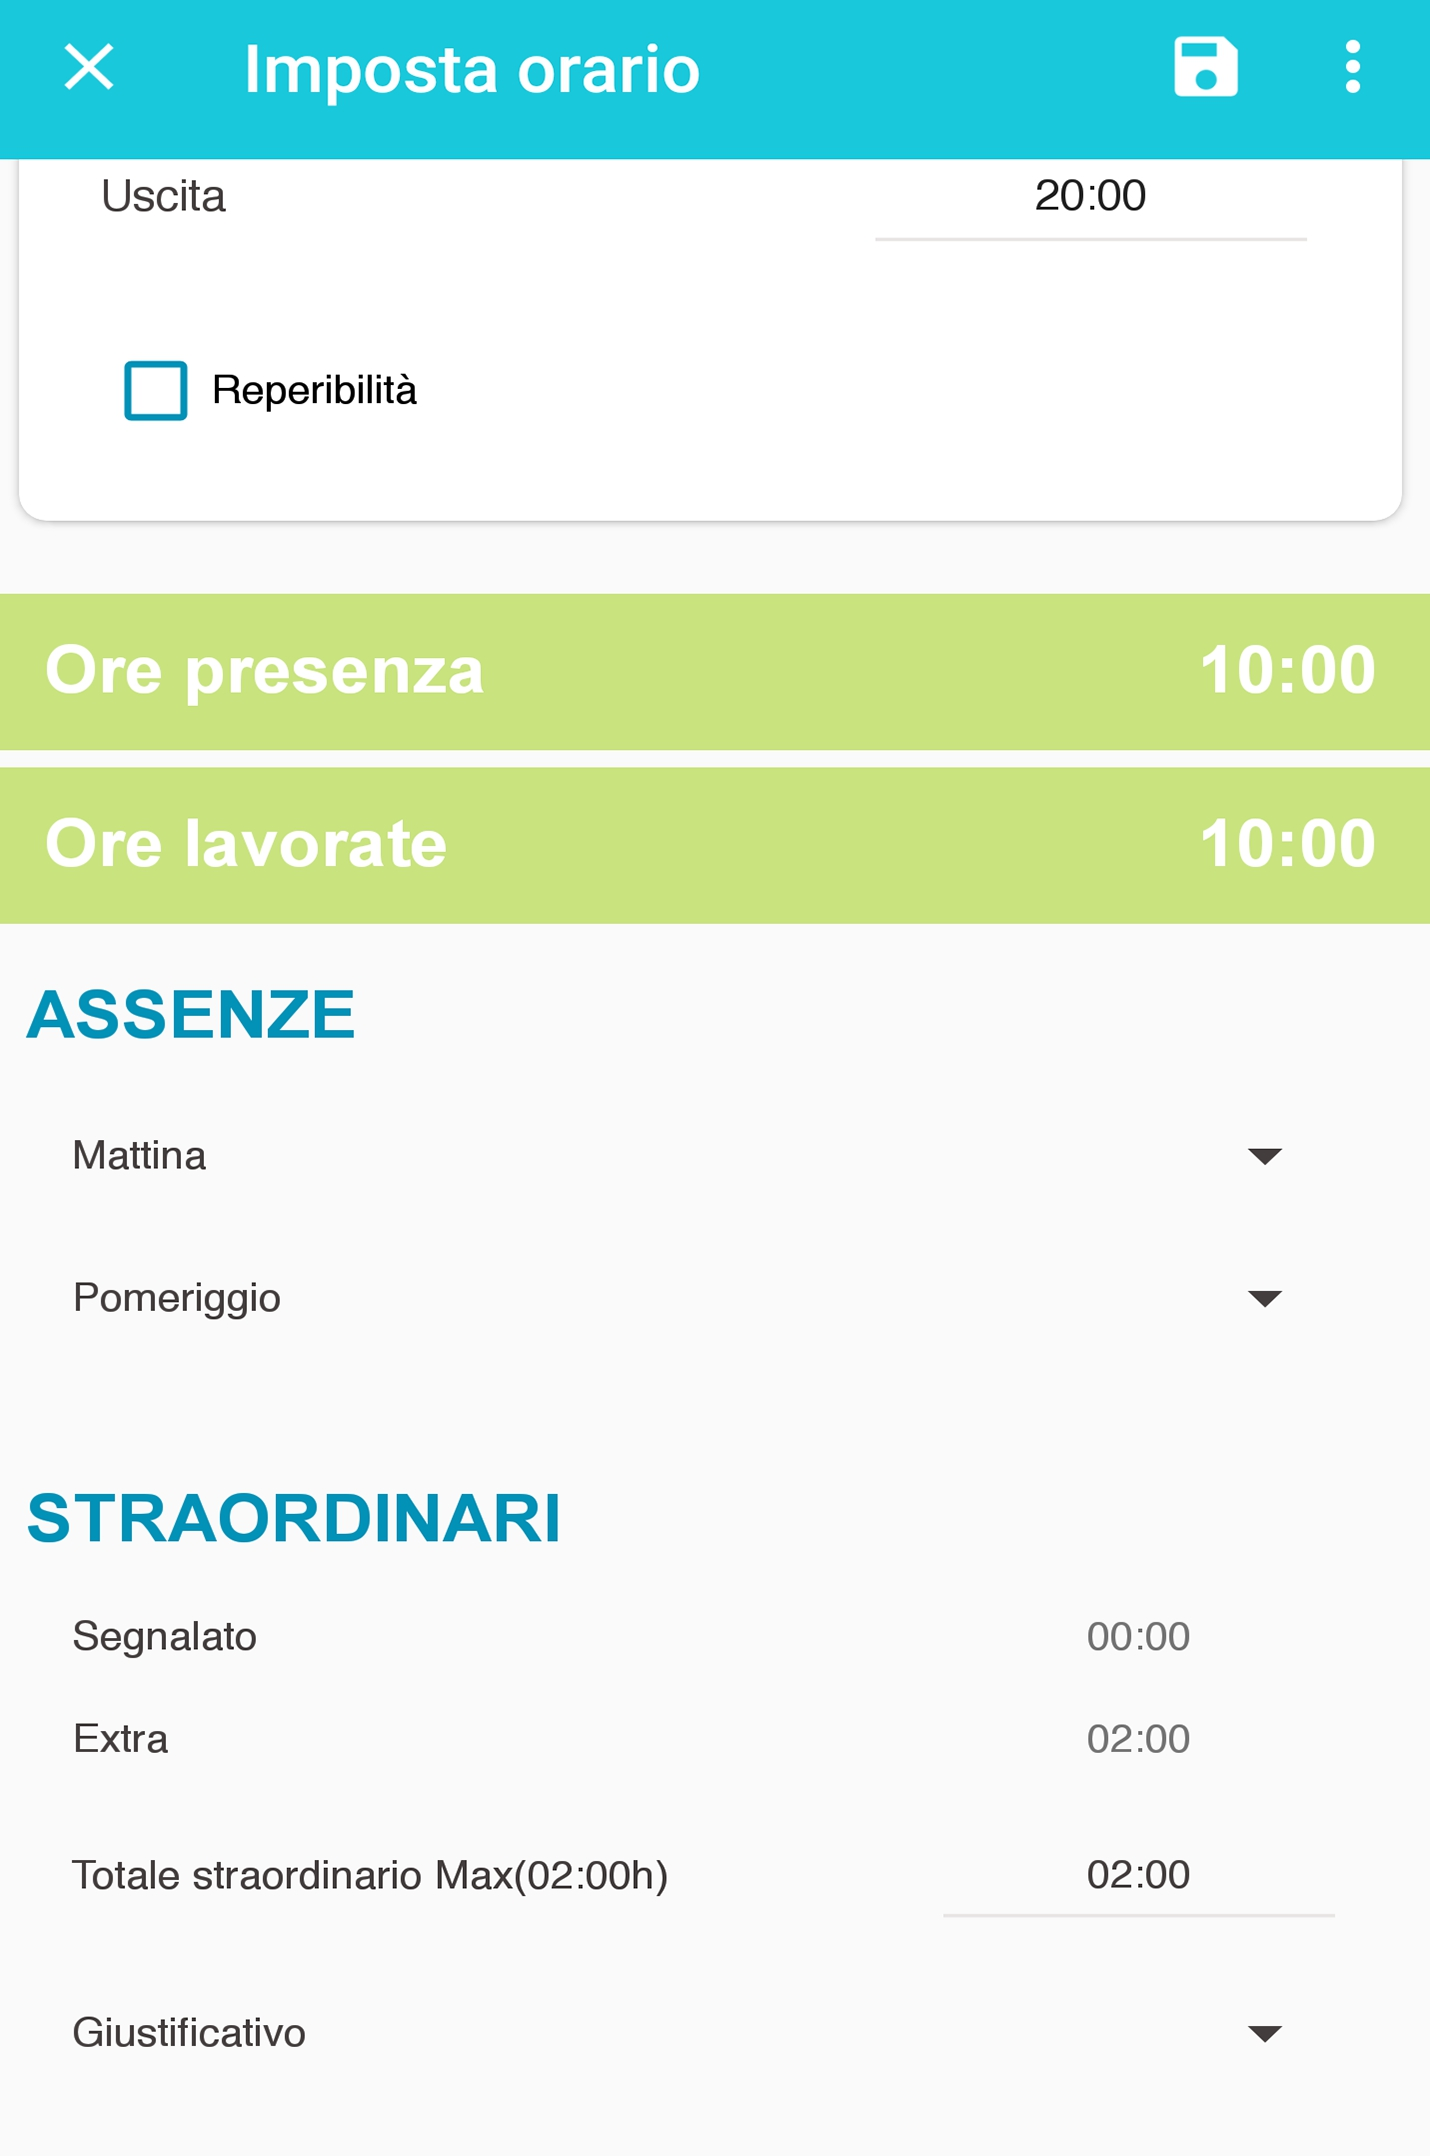
\includegraphics[width=0.8\linewidth]{immagini/timbrature_dettaglio}
	\caption{}
	\label{fig:timbraturedettaglio}
\end{figure}
\end{multicols}

La schermata delle timbrature \ref{fig:timbrature} è accessibile premendo il bottone di dettaglio della schermata principale. Tramite una lista è possibile visualizzare i propri ingressi ed uscite. Tramite la pressione di un elemento della lista è possibile eliminare una timbratura. Il pulsante \textit{timbra} permette di impostare automaticamente, in base al proprio orario di contratto, una timbratura di ingresso e uscita. Solitamente 8:30 - 12:30 / 14:00 - 18:00. Il pulsante \textit{imposta orario} permette di accedere alla schermata di dettaglio \ref{fig:timbraturedettaglio}, la quale contiene maggiori informazioni riguardanti gli orari di presenza e permette di impostare assenze, reperibilità e straordinari con i relativi giustificativi.
\newpage
\begin{multicols}{2}
	\begin{figure}[H]
	\centering
	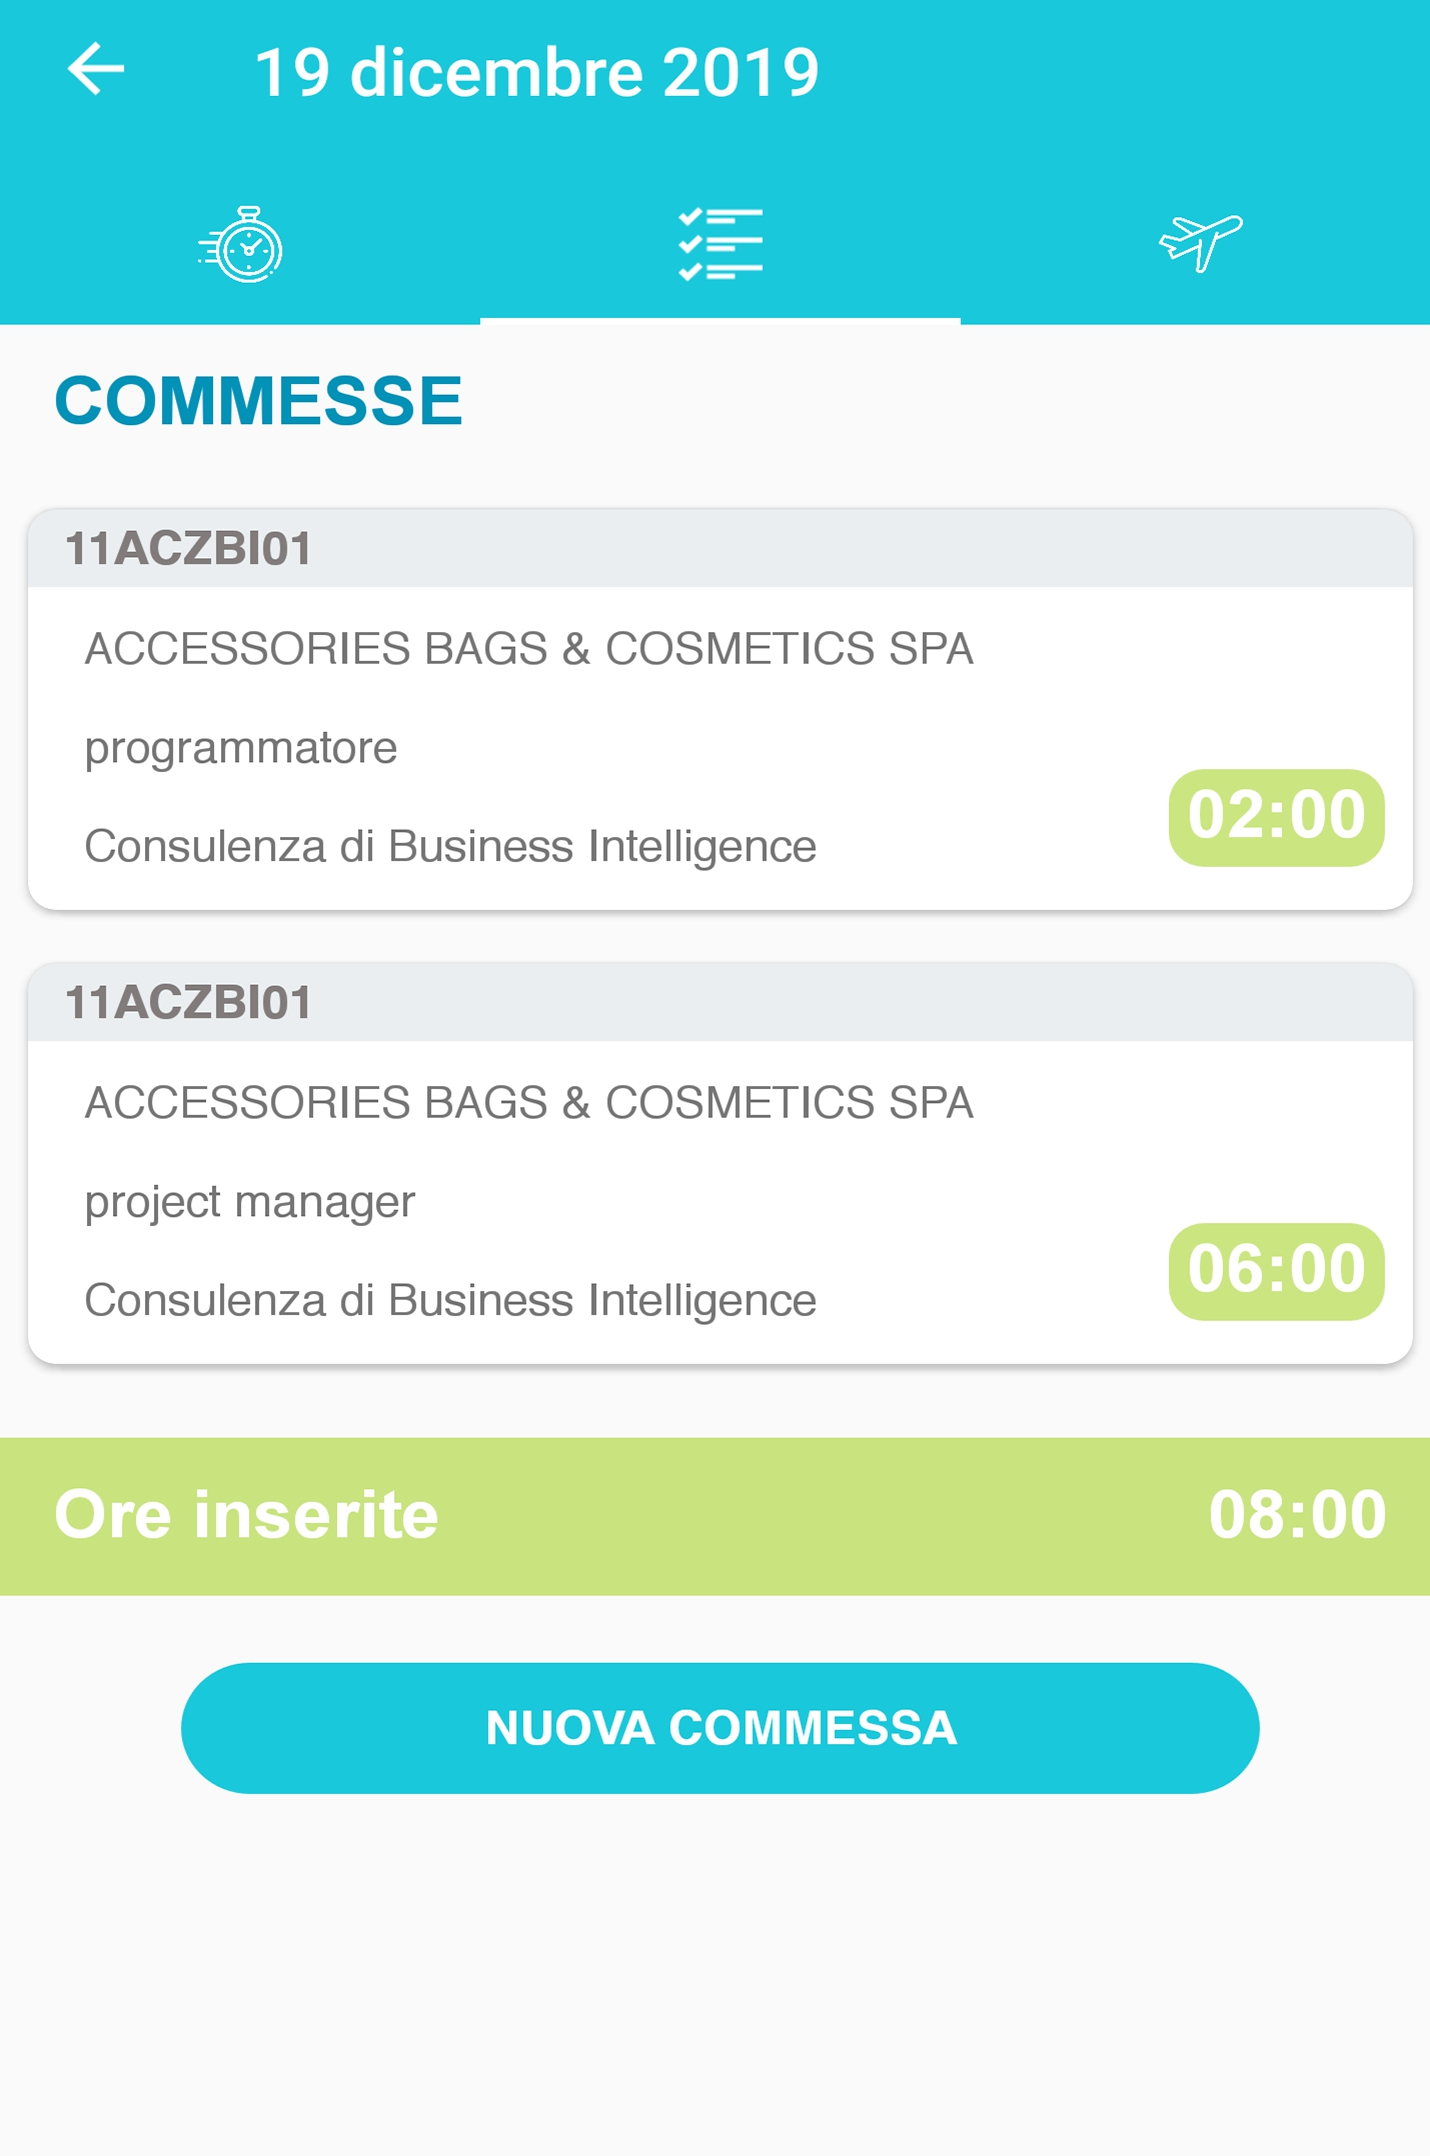
\includegraphics[width=0.8\linewidth]{immagini/commesse}
	%\caption{Prima figura}%
	\caption{}
	\label{fig:commesse}
	\end{figure}
	\begin{figure}[H]
			\centering
		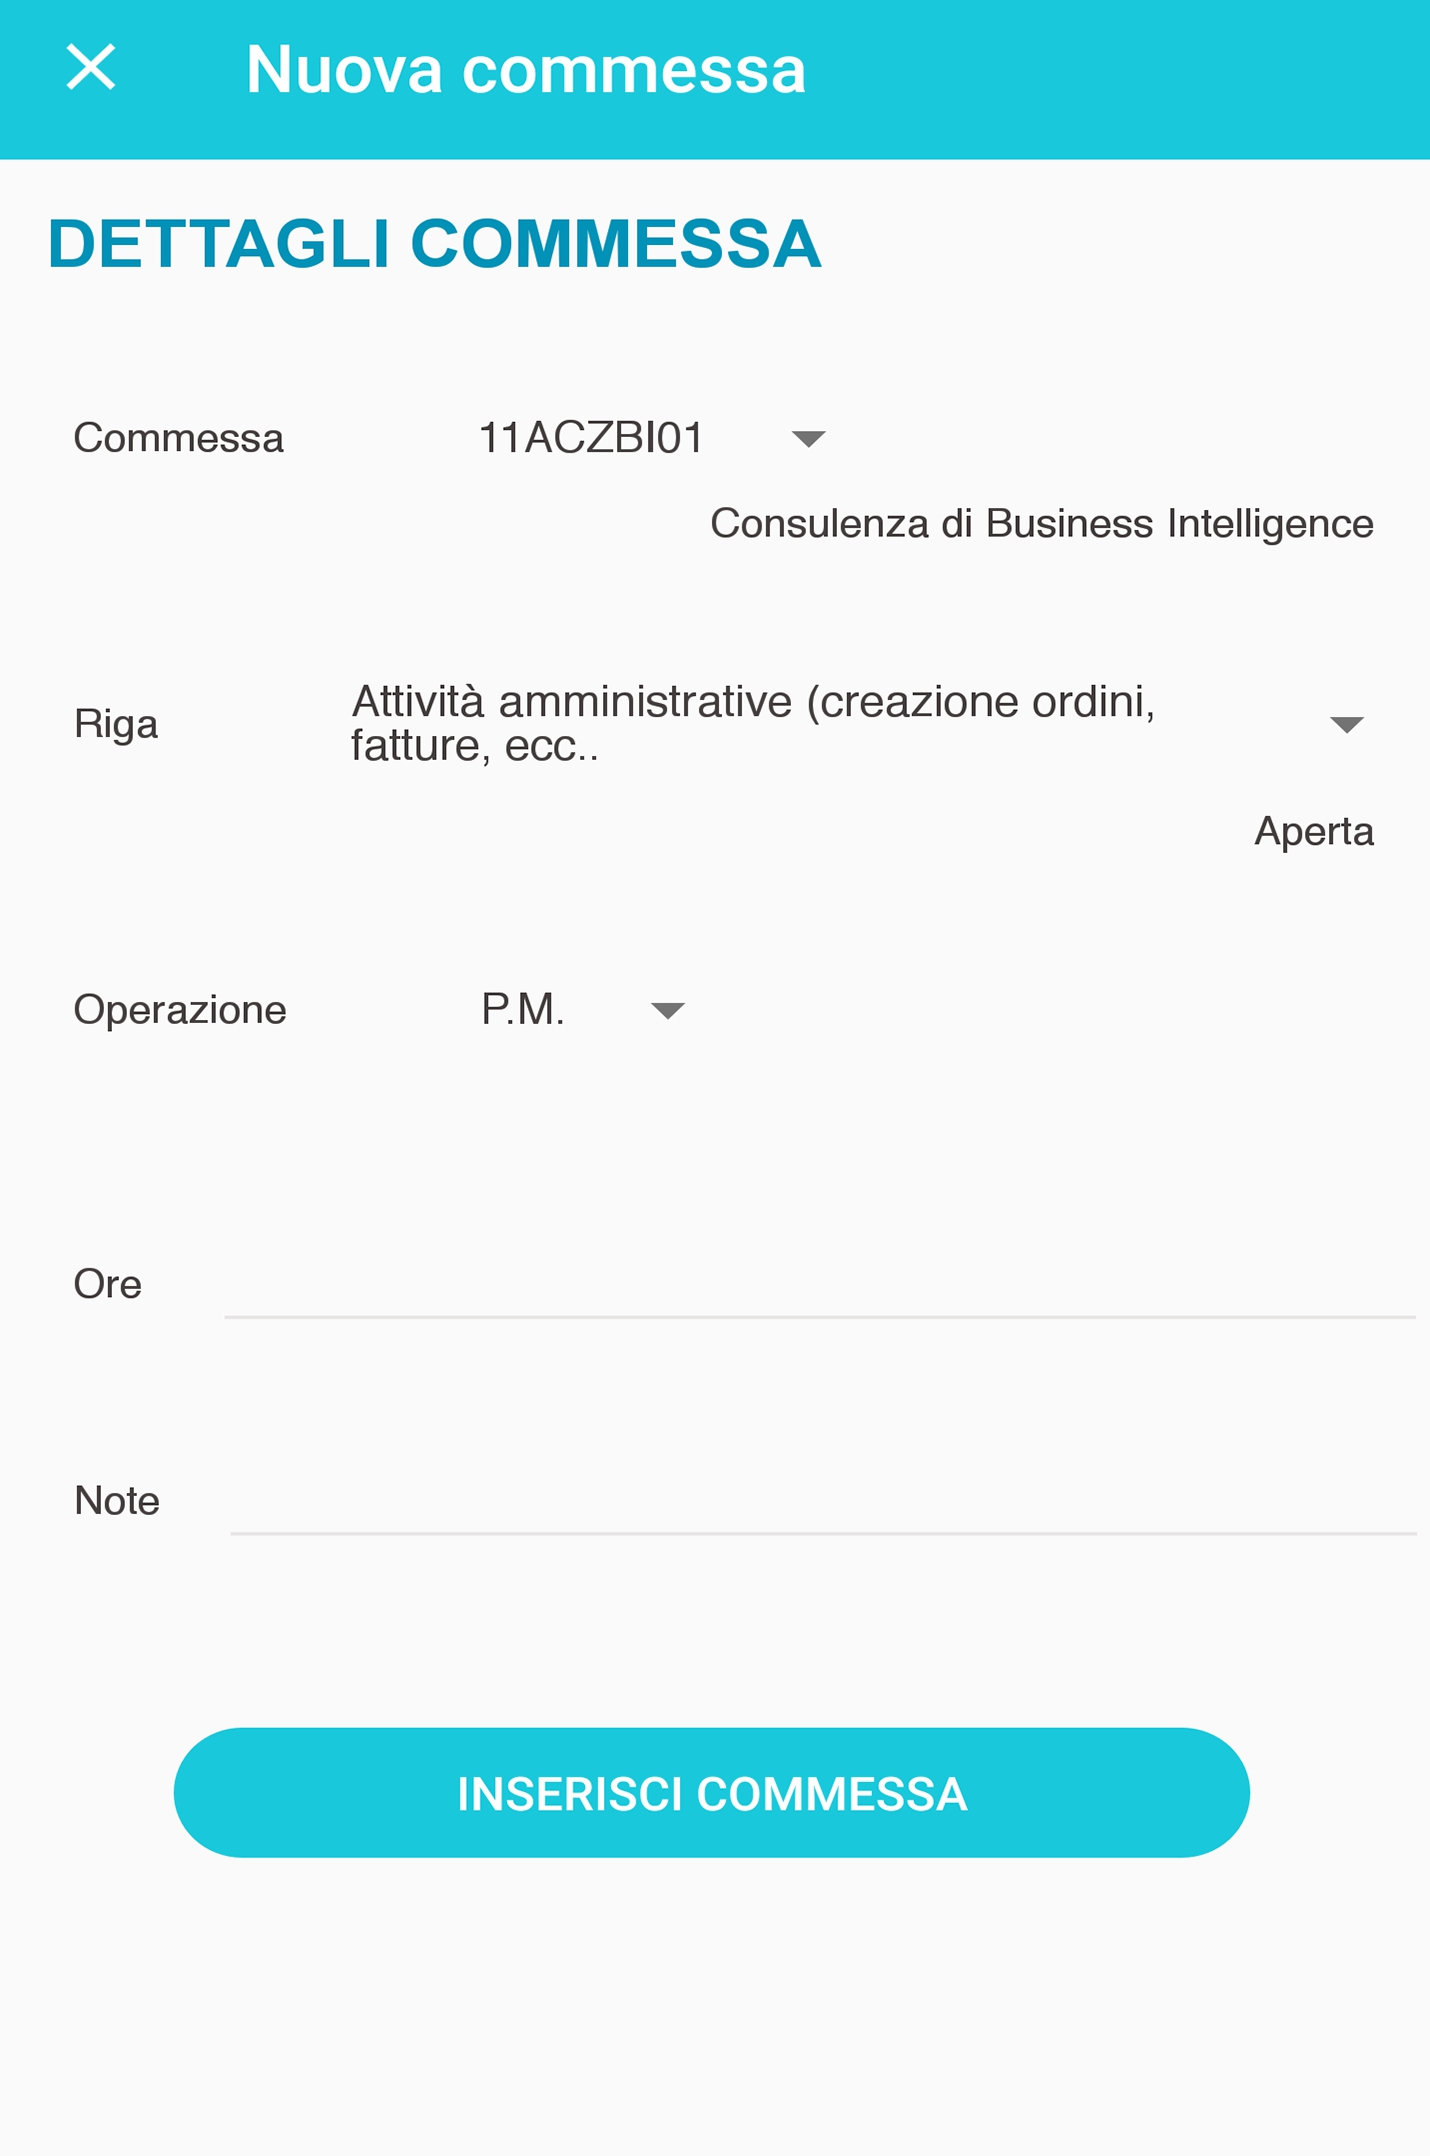
\includegraphics[width=0.8\linewidth]{immagini/commesse_dettaglio}
		\caption{}
		\label{fig:commessedettaglio}
	\end{figure}
\end{multicols}
La schermata delle commesse \ref{fig:commesse} viene visualizzata se l'utente effettua uno scorrimento a sinistra (swipe da destra a sinistra) dalla schermata delle timbrature.
Nell'interfaccia è presente una barra che mostra il numero totale di ore inserite, se la somma delle ore coincide con il numero di ore lavorate sarà di colore verde, altrimenti rossa.
% L'interfaccia permette di visualizzare gli ordini inseriti durante la giornata selezionata, se la somma delle ore coincide con il numero di ore che il dipendente deve lavorare in una giornata la barra sarà verde altrimenti rossa.
Tramite un tap sarà possibile eliminare una commessa. Il bottone \textit{nuova commessa} apre una schermata di dettaglio (figura \ref{fig:commessedettaglio}) che permette di inserire un nuovo ordine impostando: numero della commessa, attività e mansione svolta, il tempo massimo impiegato per svolgere un determinato ordine ed eventuali note.

\begin{figure}[!h]
	\centering
	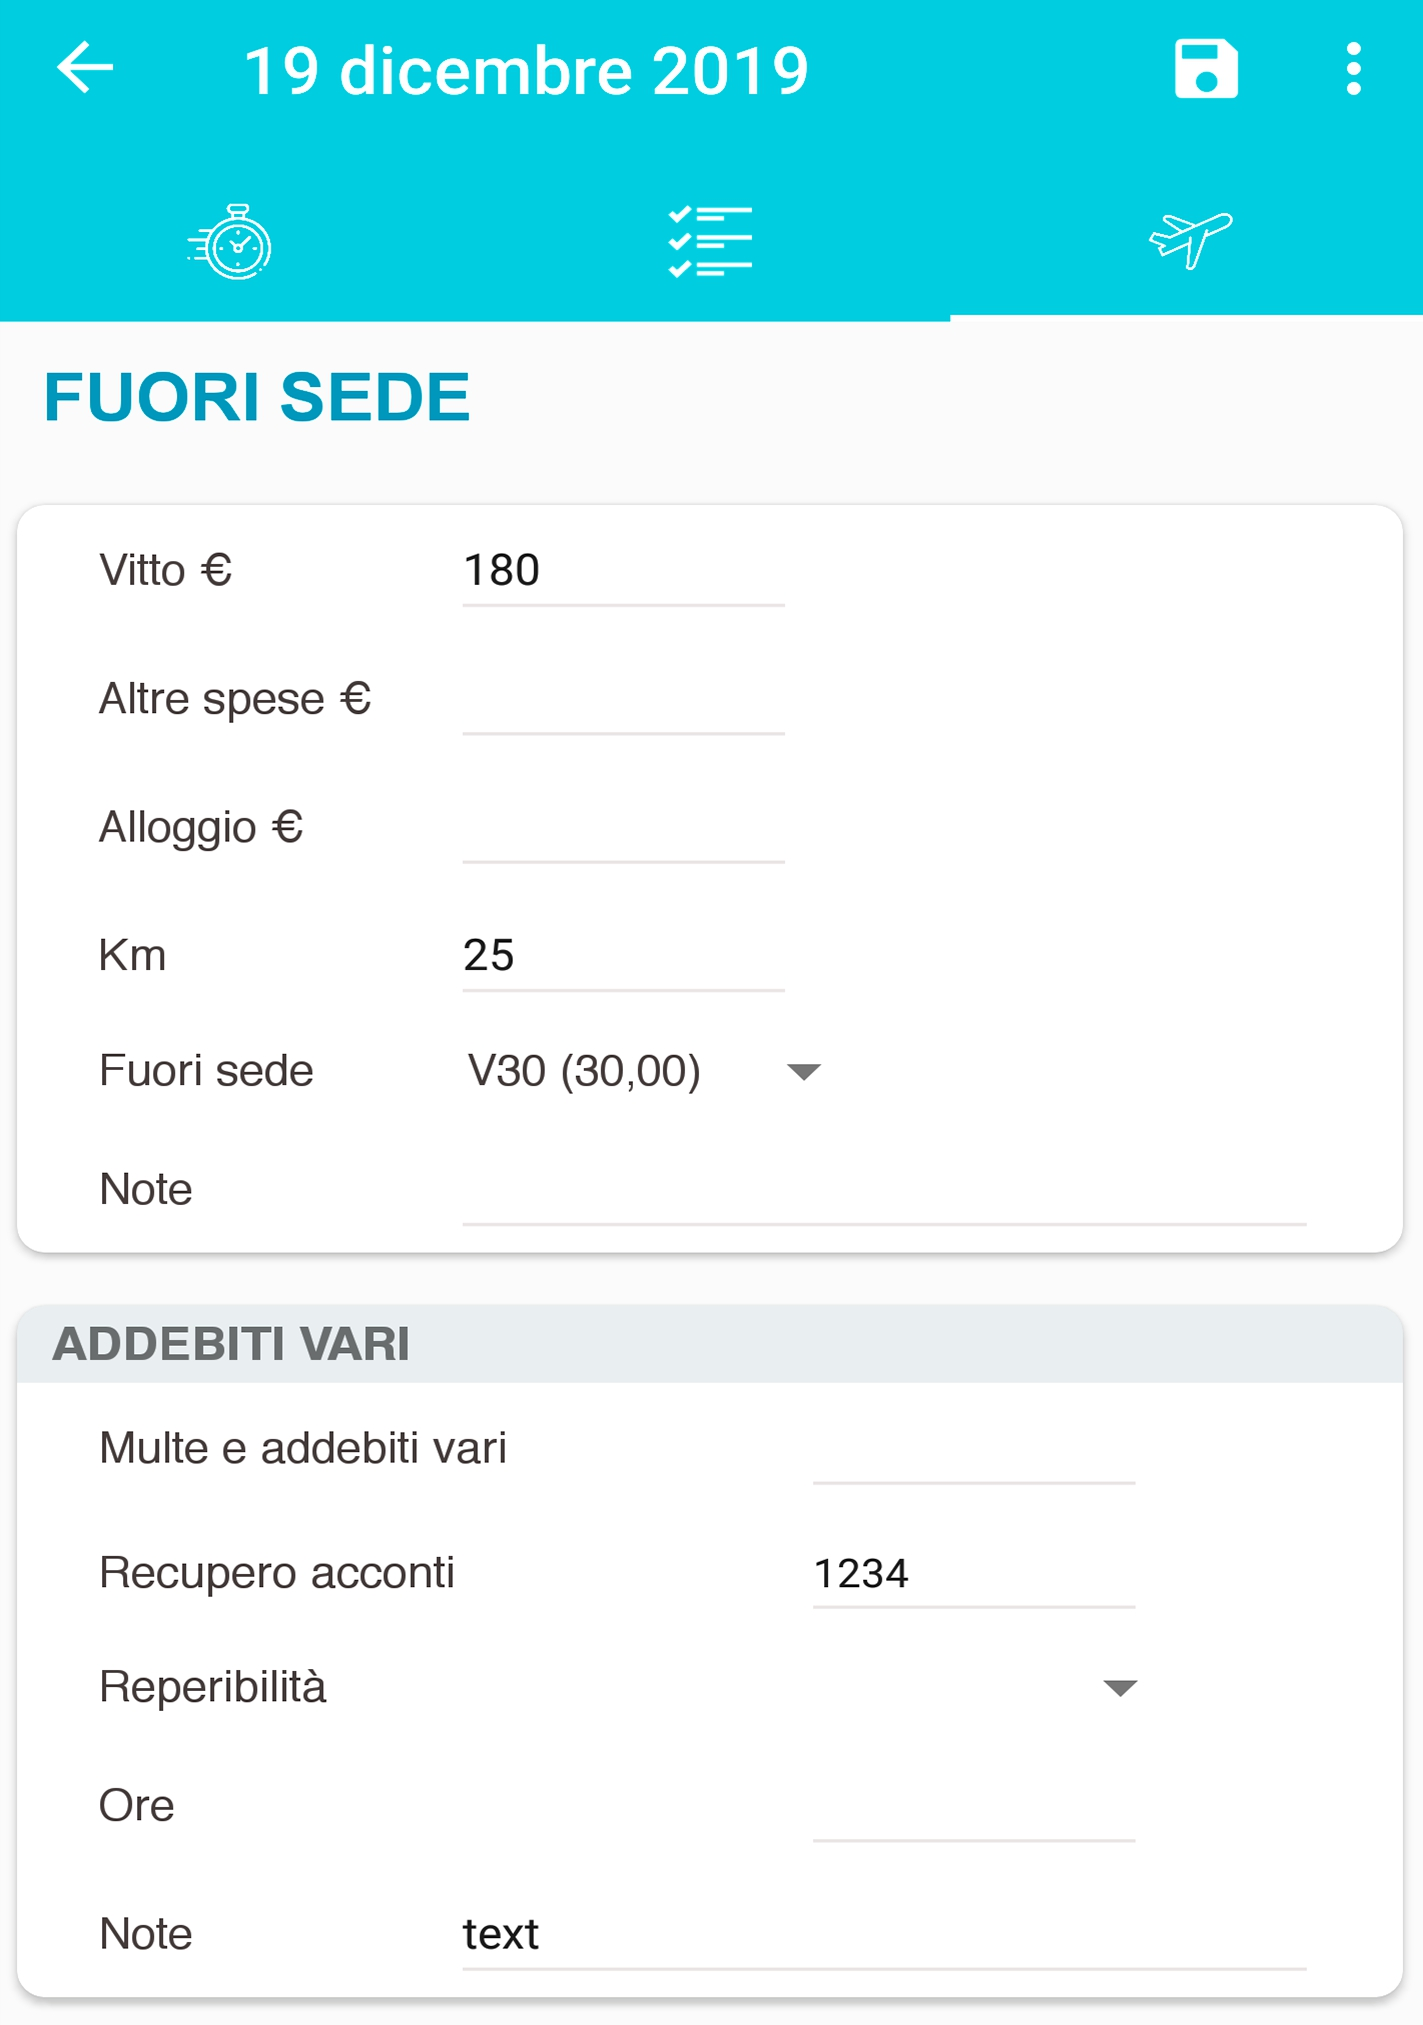
\includegraphics[width=0.4\linewidth]{immagini/trasferte}
	\caption{}
	\label{fig:trasferte}
\end{figure}
L'ultima schermata che l'utente può visualizzare all'interno del dettaglio è quella delle trasferte (figura \ref{fig:trasferte}). Per accedervi l'utente dovrà effettuare due swipe a destra dalla schermata delle timbrature oppure tramite il tab layout selezionare l'icona che rappresenta la schermata. L'interfaccia permette di inserire le spese effettuate dai dipendenti per motivi lavorativi al di fuori dell'azienda.
\newpage
L'ordine delle schermate è stato impostato visualizzando per prima quella che più utenti utilizzeranno, e per ultima la meno utilizzata, in modo tale che la maggior parte di essi possa svolgere i propri task nel minor tempo possibile. Di seguito viene mostrato l'ordine di visualizzazione delle schermate.
	\begin{center}
	Timbrature \textrightarrow{} Commesse \textrightarrow{} Rimborso spese
	\end{center}
\section{User flow}
Lo User flow è un diagramma che rappresenta come l'utente navigherà all'interno dell'applicazione. Implementare un buon flusso di navigazione è importante perchè permette agli utenti di raggiungere gli obiettivi in modo semplice e veloce. Ad esempio, la richiesta di troppe informazioni in una schermata di login può scoraggiare l'utente a registrarsi e quindi non raggiungere l'obiettivo finale, per questo è importante organizzare le informazioni in modo chiaro e ordinato.\\
Durante la realizzazione dei prototipi quando veniva aggiunta, modificata o rimossa una schermata si analizzava lo user flow risultante. Grazie a questo diagramma è stato possibile verificare l'esperienza utente complessiva e valutare se modificare o meno alcuni componenti di interazione come: bottoni, campi di inserimento, campi di selezione, ecc.. così da rendere il flusso di navigazione intuitivo e scorrevole per l'utente, permettendogli di raggiungere l'obiettivo nel minor tempo possibile. Di seguito viene riportato il task flow finale ottenuto dallo studio appena descritto.

\begin{figure}[h!]
	\centering
	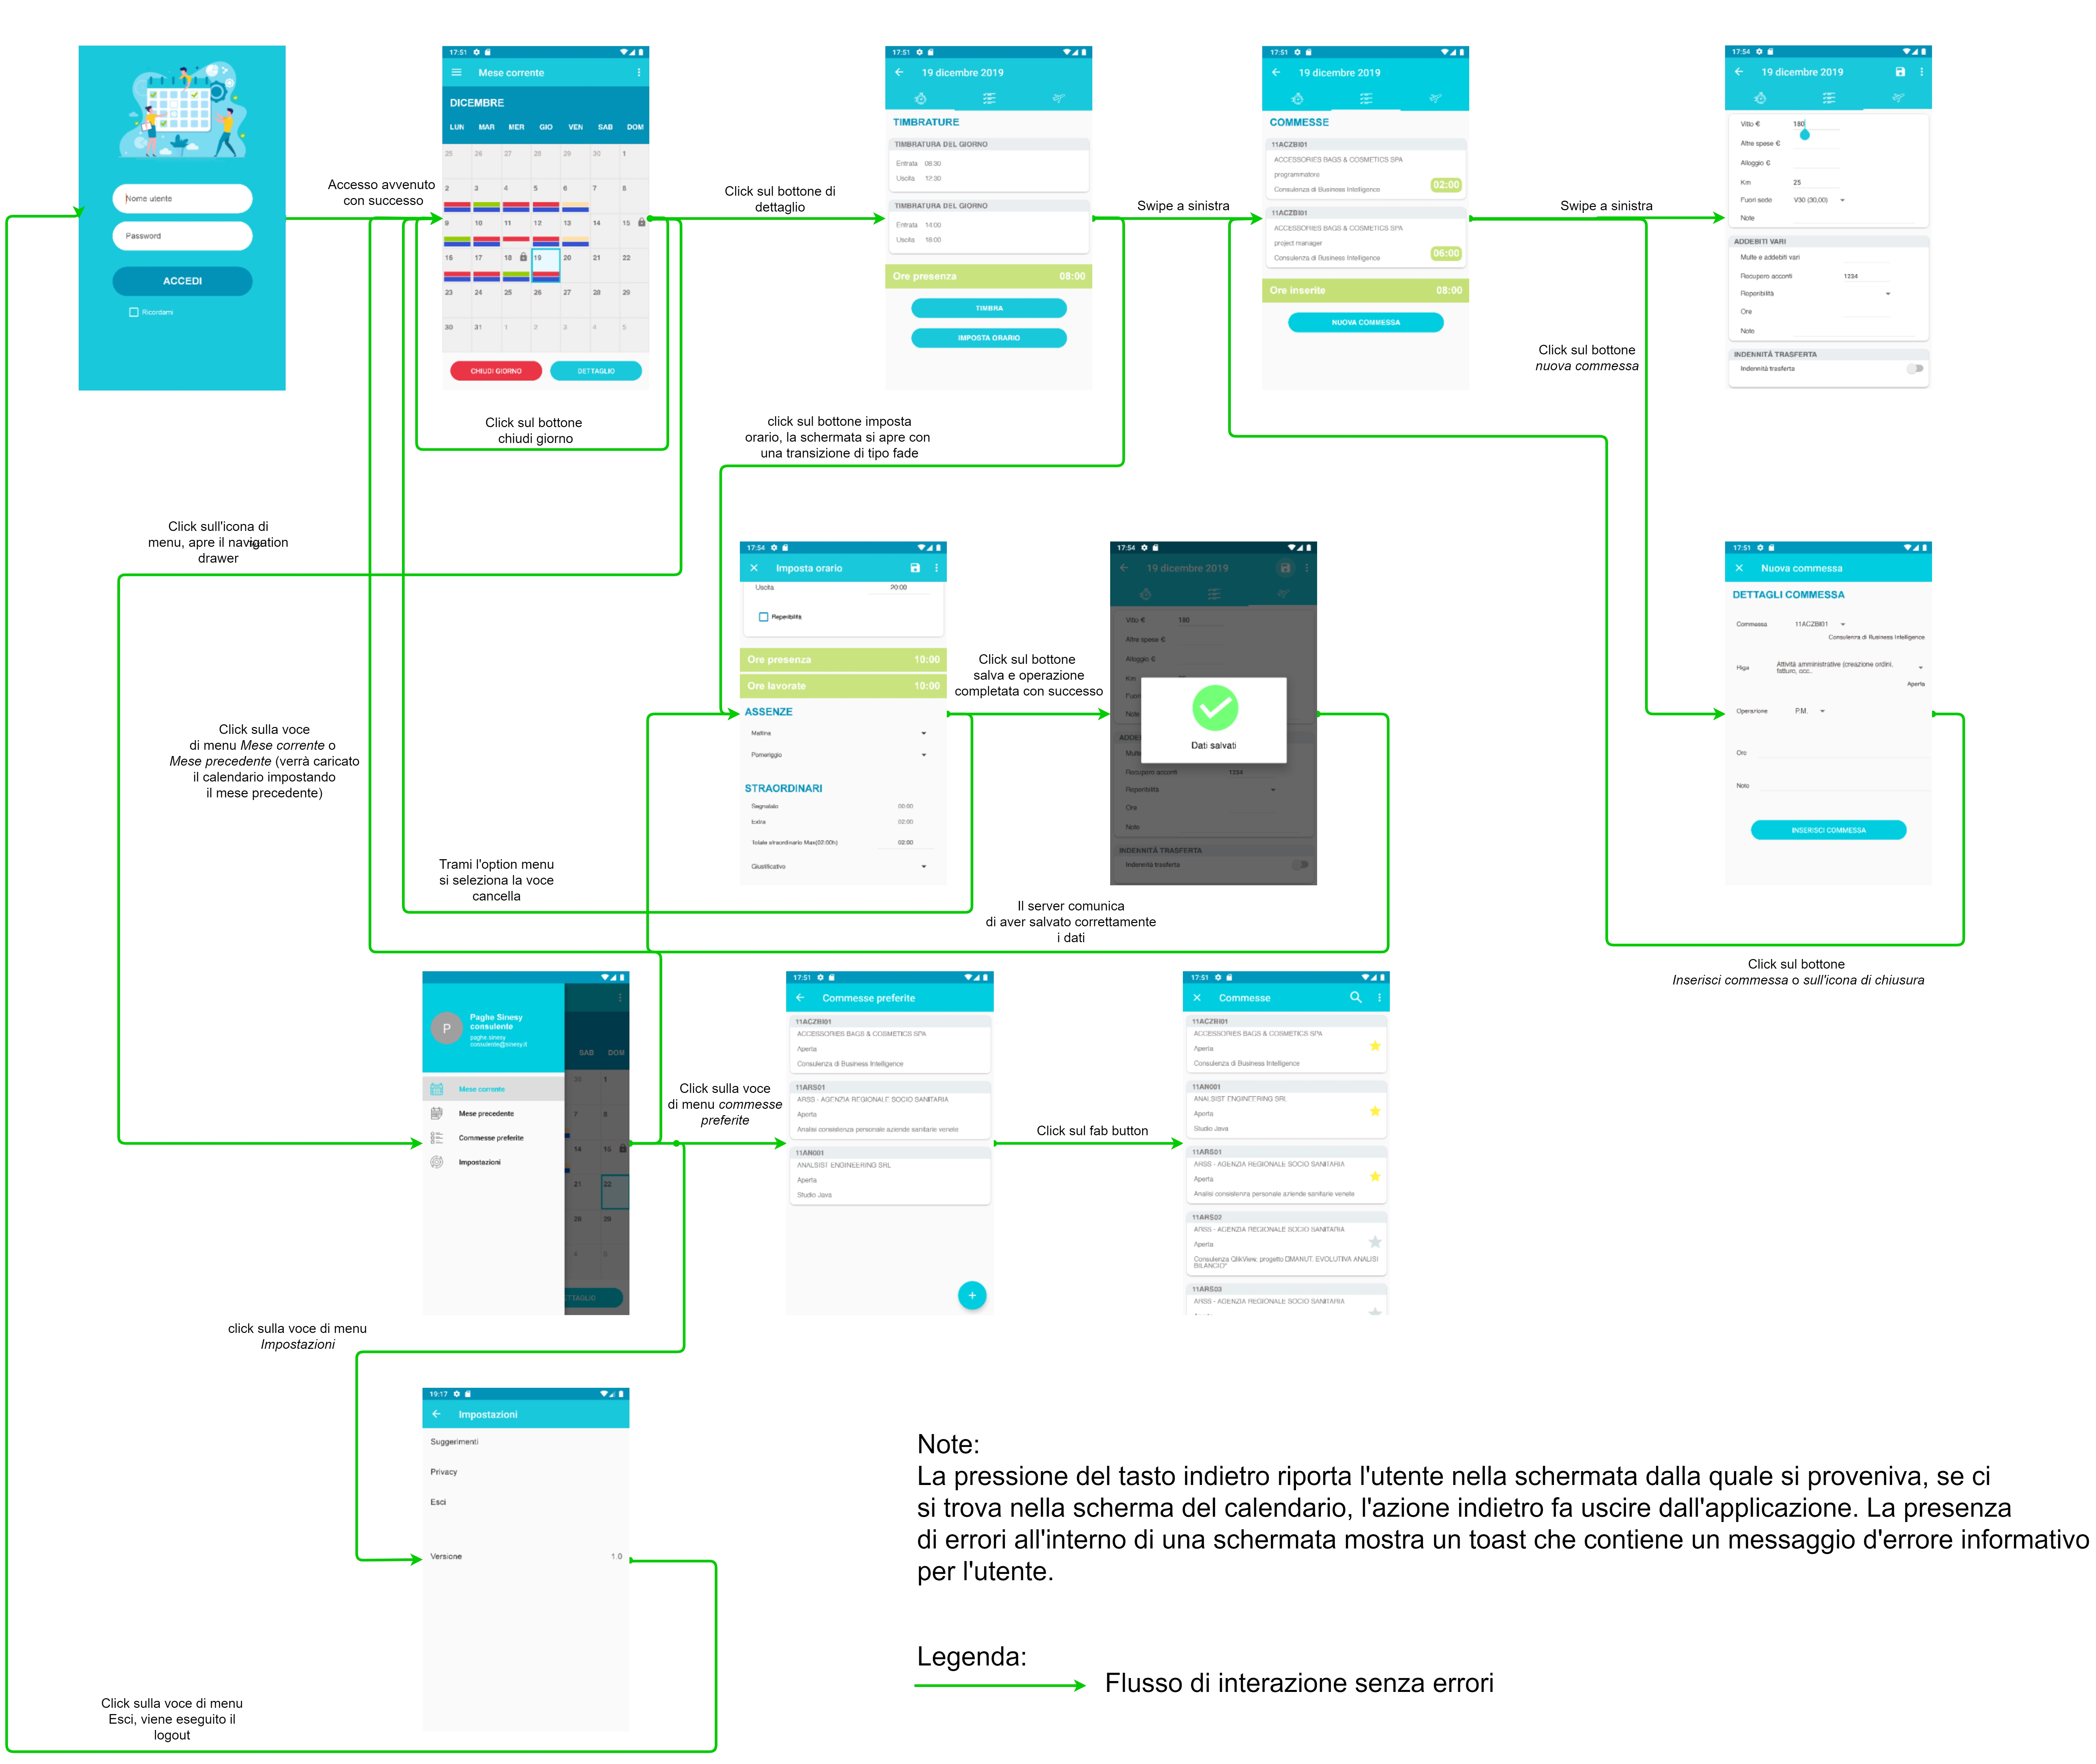
\includegraphics[width=1.1\linewidth]{immagini/UserFlow}
	\caption{User flow finale}
\end{figure}
\newpage
\section{Ottimizzazione dei flussi}
Durante il processo di progettazione si è deciso di ottimizzare alcuni flussi di interazione perchè considerati azioni frequenti svolte da ogni utente. 
\begin{multicols}{2}
	\begin{figure}[H]
		\centering
		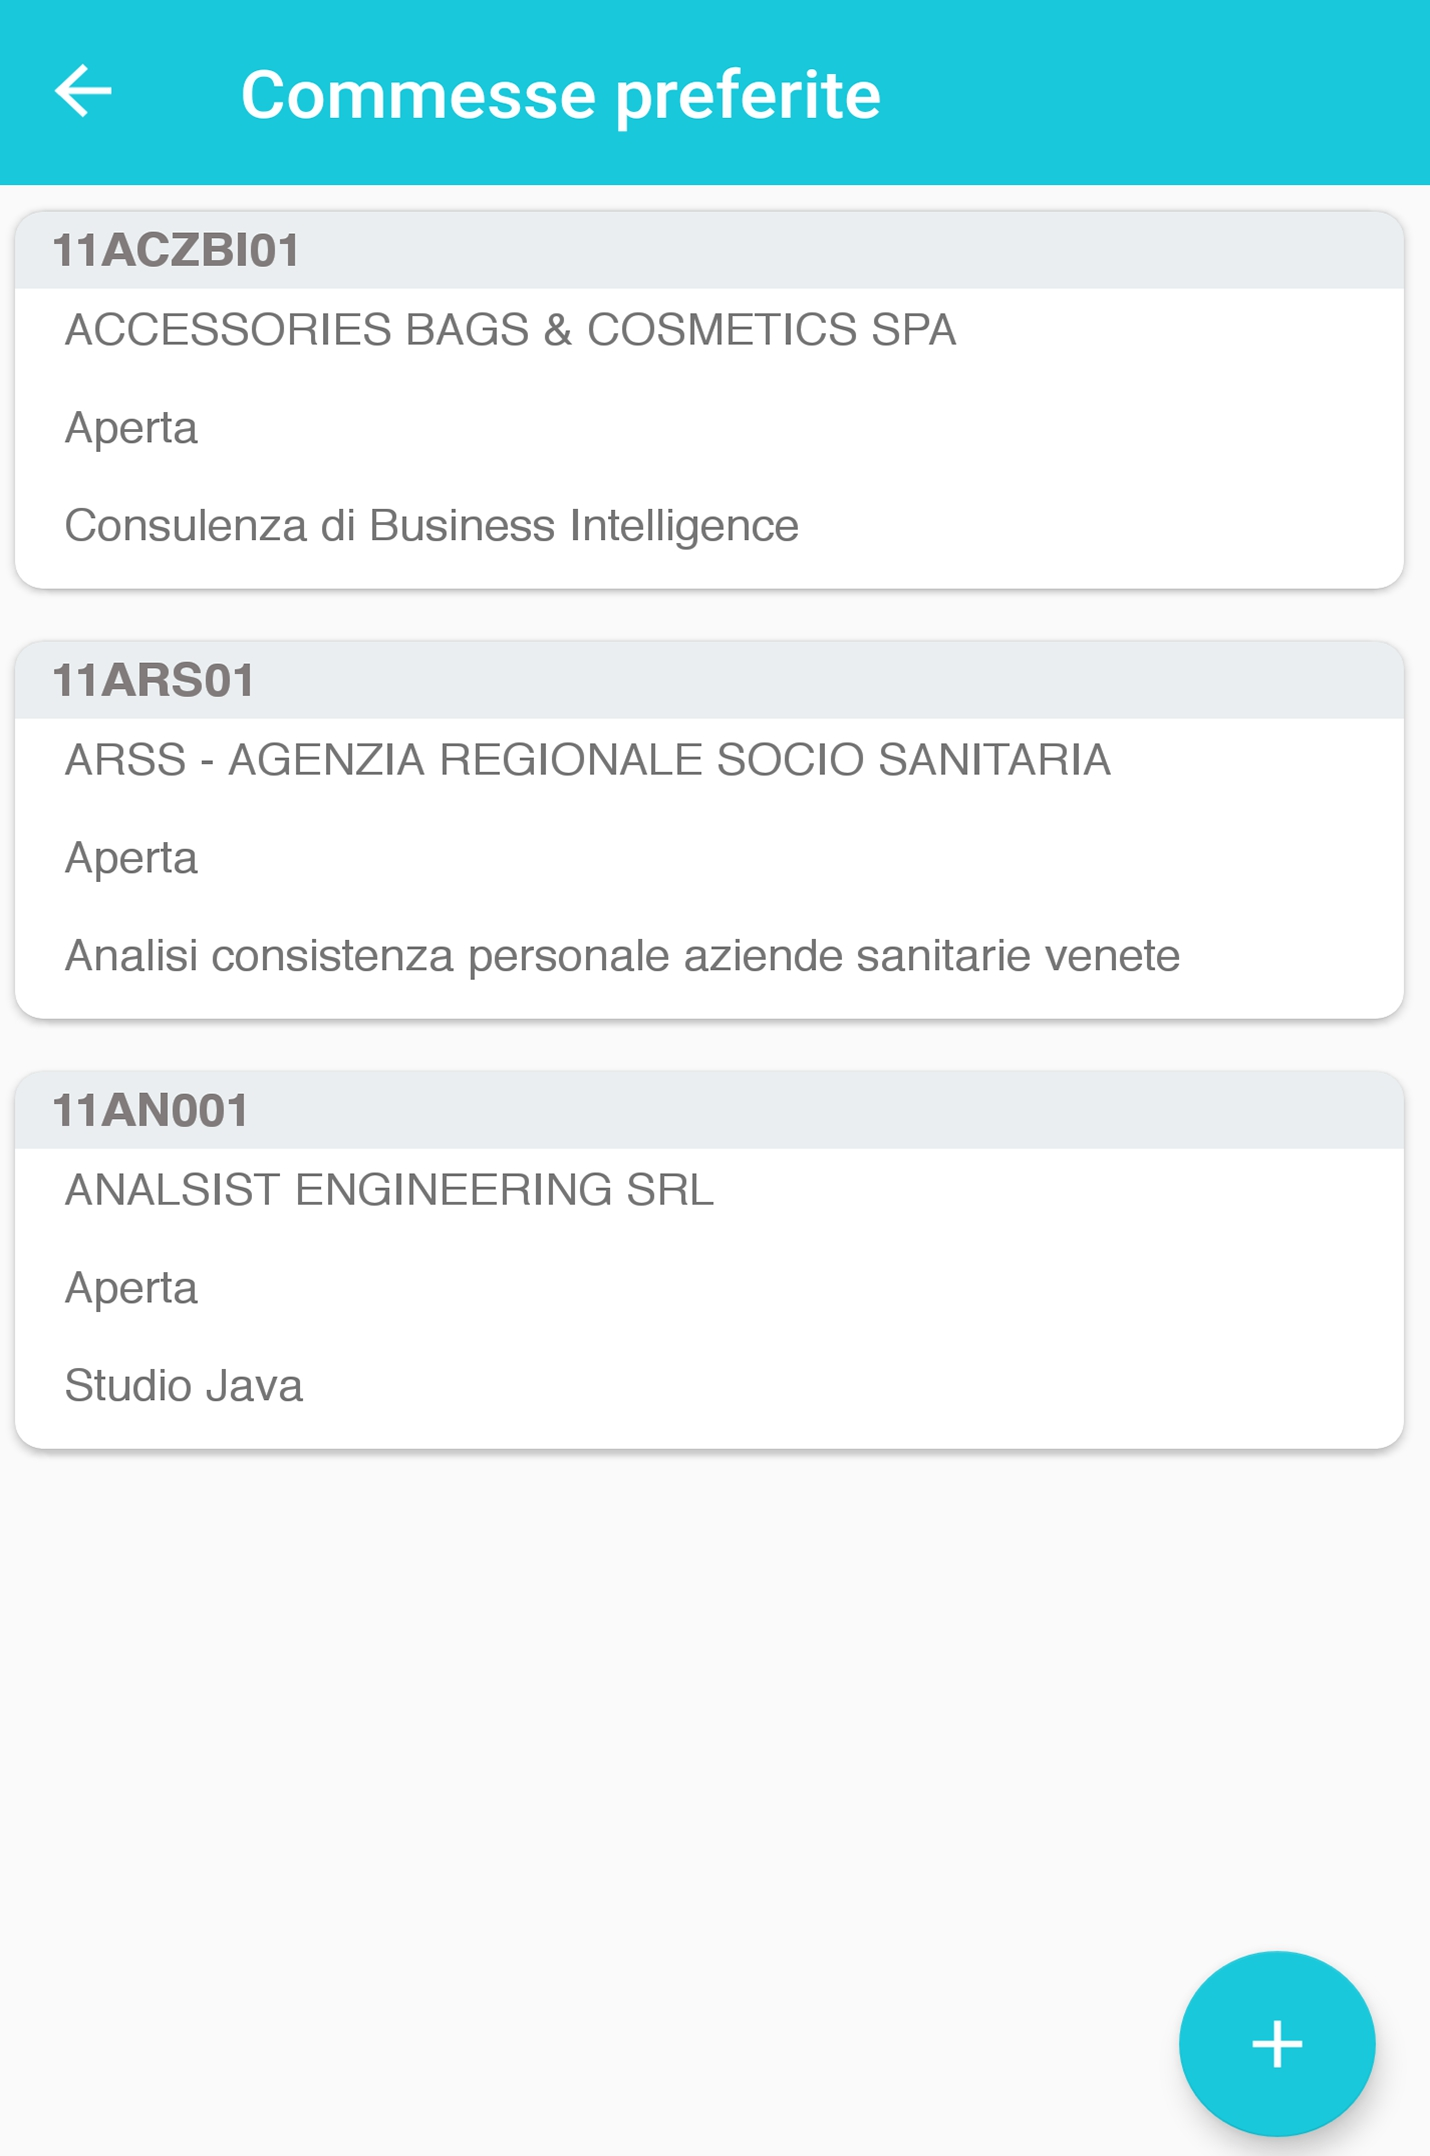
\includegraphics[width=0.8\linewidth]{immagini/commesse_pref}
		\caption{}
		\label{fig:commessepref}
	\end{figure}
	\begin{figure}[H]
		\centering
		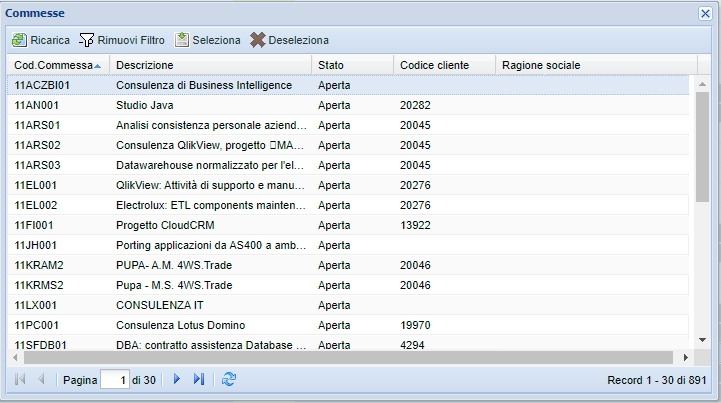
\includegraphics[width=1.2\linewidth]{immagini/inserimento commessa}
		\caption{}
		\label{fig:inscommessa}
	\end{figure}
\end{multicols}

Il primo flusso è \textit{l'inserimento delle commesse}. Ogni giorno un dipendente deve inserire potenzialmente [1,n] ordini. Valutando le commesse inserite mediamente nella piattaforma web è emerso che un dipendente lavora di media a [1,5] progetti in un mese. Viene quindi introdotta una finestra \ref{fig:commessepref} per permettere di salvare le commesse alle quali si lavora più di frequente, in questo modo l'utente potrà accedere rapidamente alle proprie commesse e non dovrà ricercarle ogni volta in una lista che contiene circa 1000 record (si veda figura \ref{fig:inscommessa}).
\newpage
\begin{multicols}{2}
	\begin{figure}[H]
		\centering
	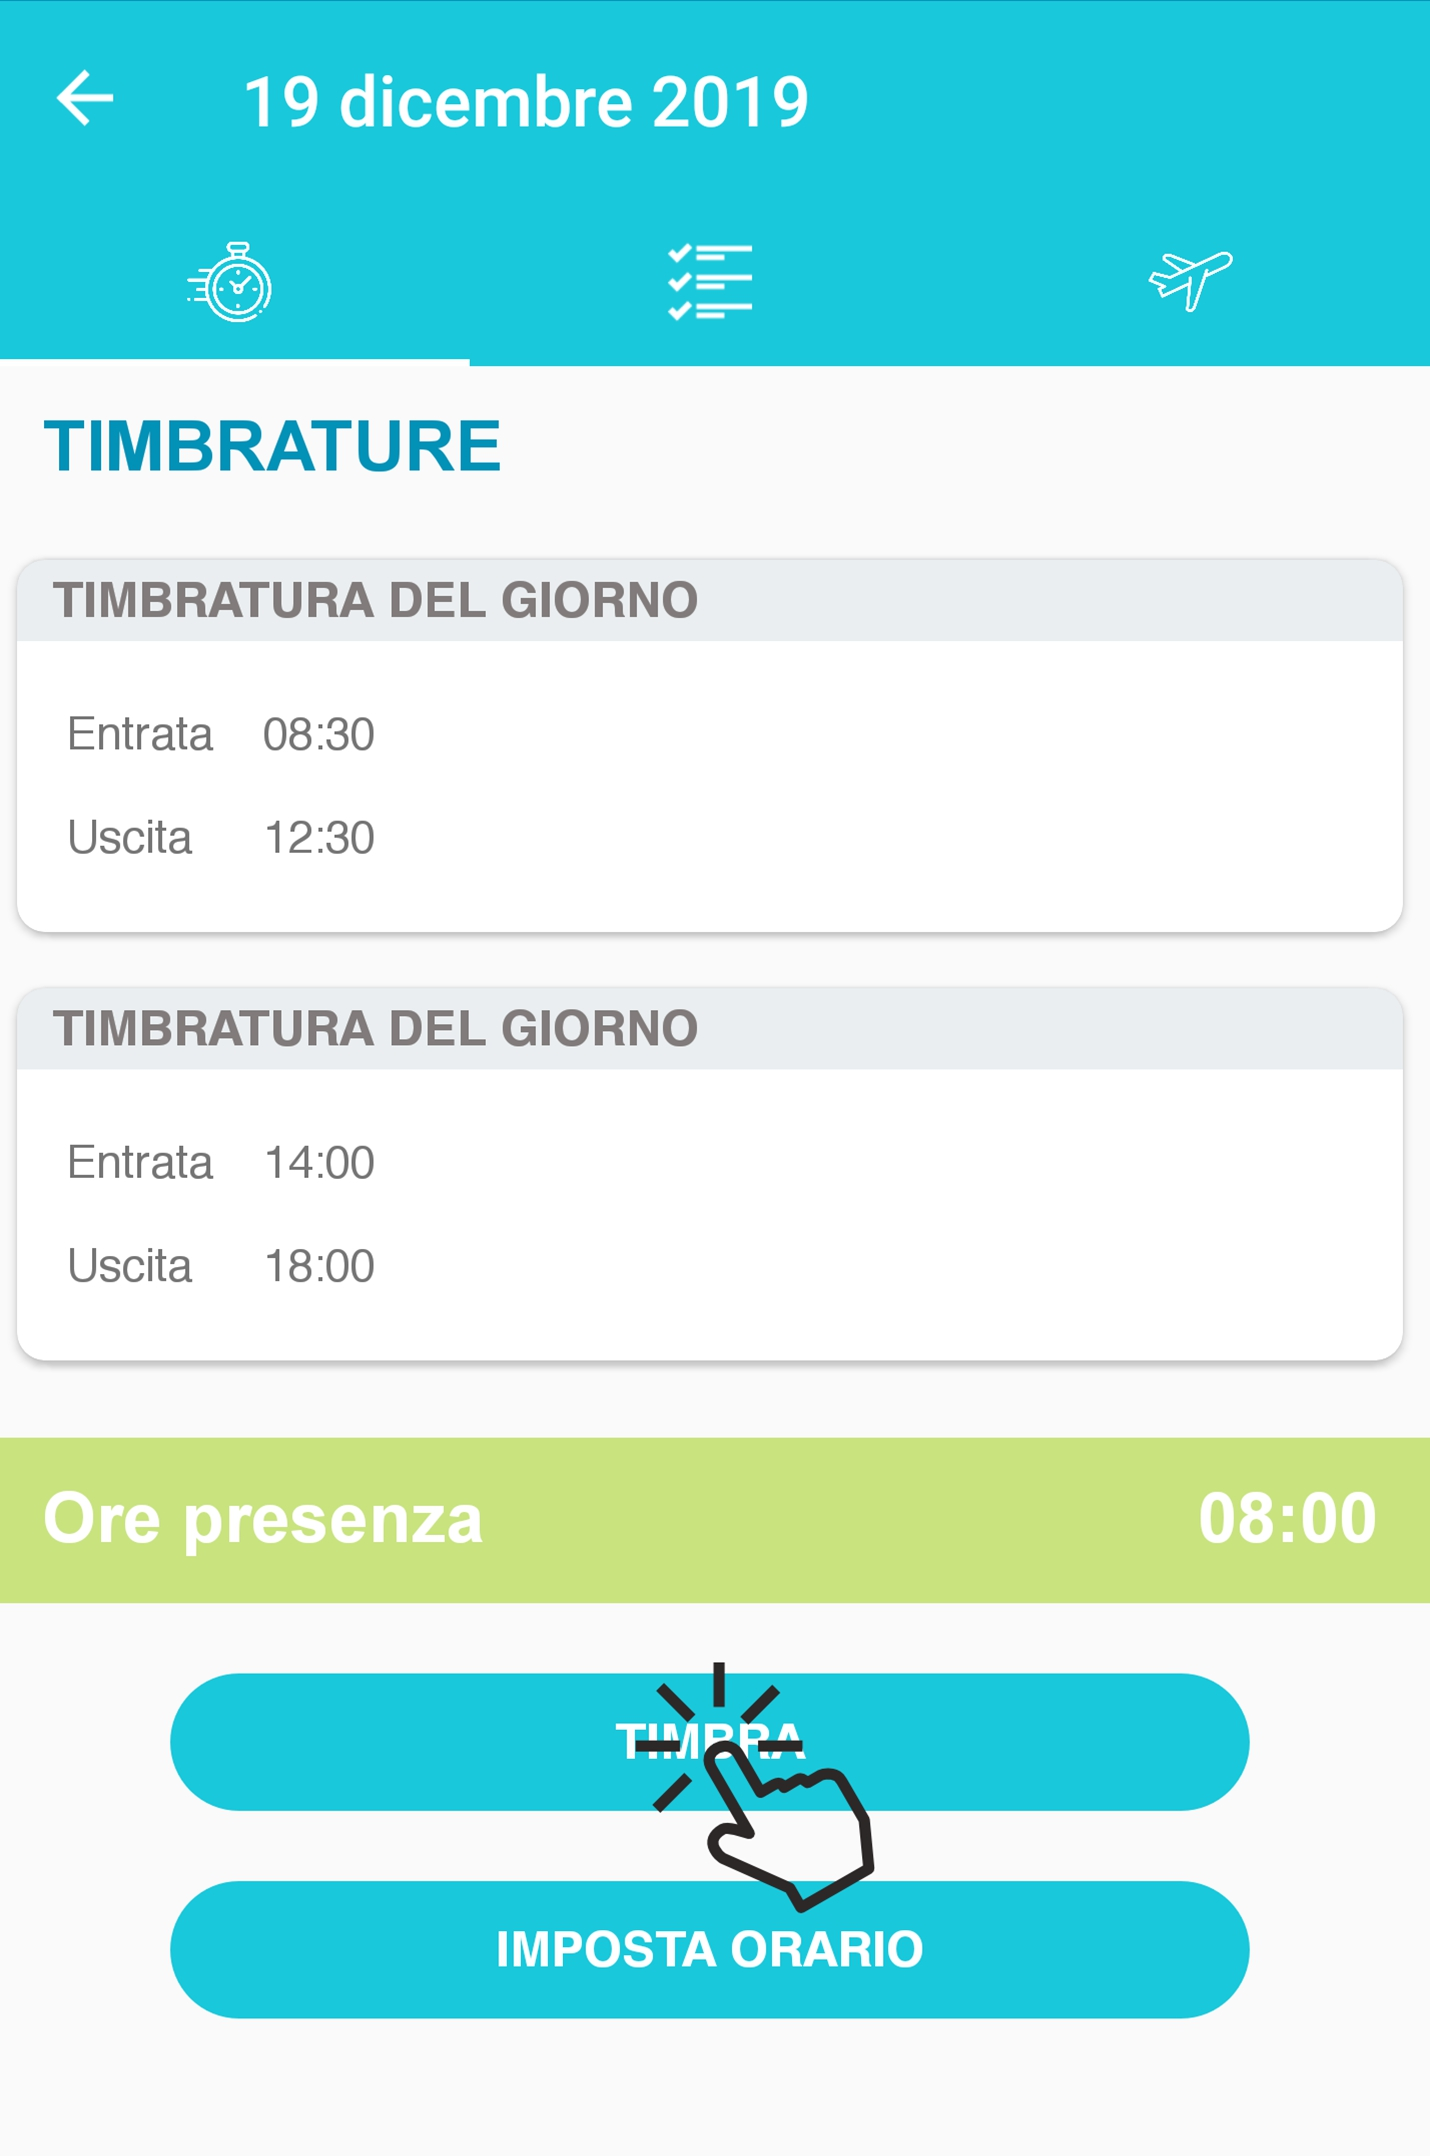
\includegraphics[width=0.7\linewidth]{immagini/timbra}
	\caption{}
	\label{fig:commessetimbra}
	\end{figure}
	\begin{figure}[H]
		\centering
	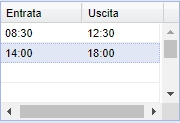
\includegraphics[width=0.6\linewidth]{immagini/inserimento orario}
	\caption{}
	\label{fig:insorario}
	\end{figure}
\end{multicols}

Il secondo flusso studiato è \textit{l'inserimento delle timbrature}. Questa operazione viene svolta giornalmente, anche più di una volta al giorno, da quasi ogni dipendente dell'azienda. Solitamente ogni lavoratore ha un orario predefinito es: 8:30 - 12:30 / 14:00 - 18:00 il quale si ripete ogni giorno lavorativo. Per evitare errori di inserimento, viene introdotto nella schermata un bottone, che permette di inserire due coppie [ingresso, uscita] che coincidono con il proprio orario di lavoro preimpostato dal sistema. Grazie a questo bottone il dipendente non dovrà più ricordarsi quali sono i suoi orari e poi inserirli manualmente in una tabella, come accadeva nella versione web (si veda figura \ref{fig:insorario}), ma con la semplice pressione del bottone \textit{timbra} l'utente inserirà le due coppie di valori associate ad esso. Grazie a questa funzionalità vengono corretti gli errori di timbrature che erano frequenti nella piattaforma web.


\begin{figure}[!h]
	\centering
	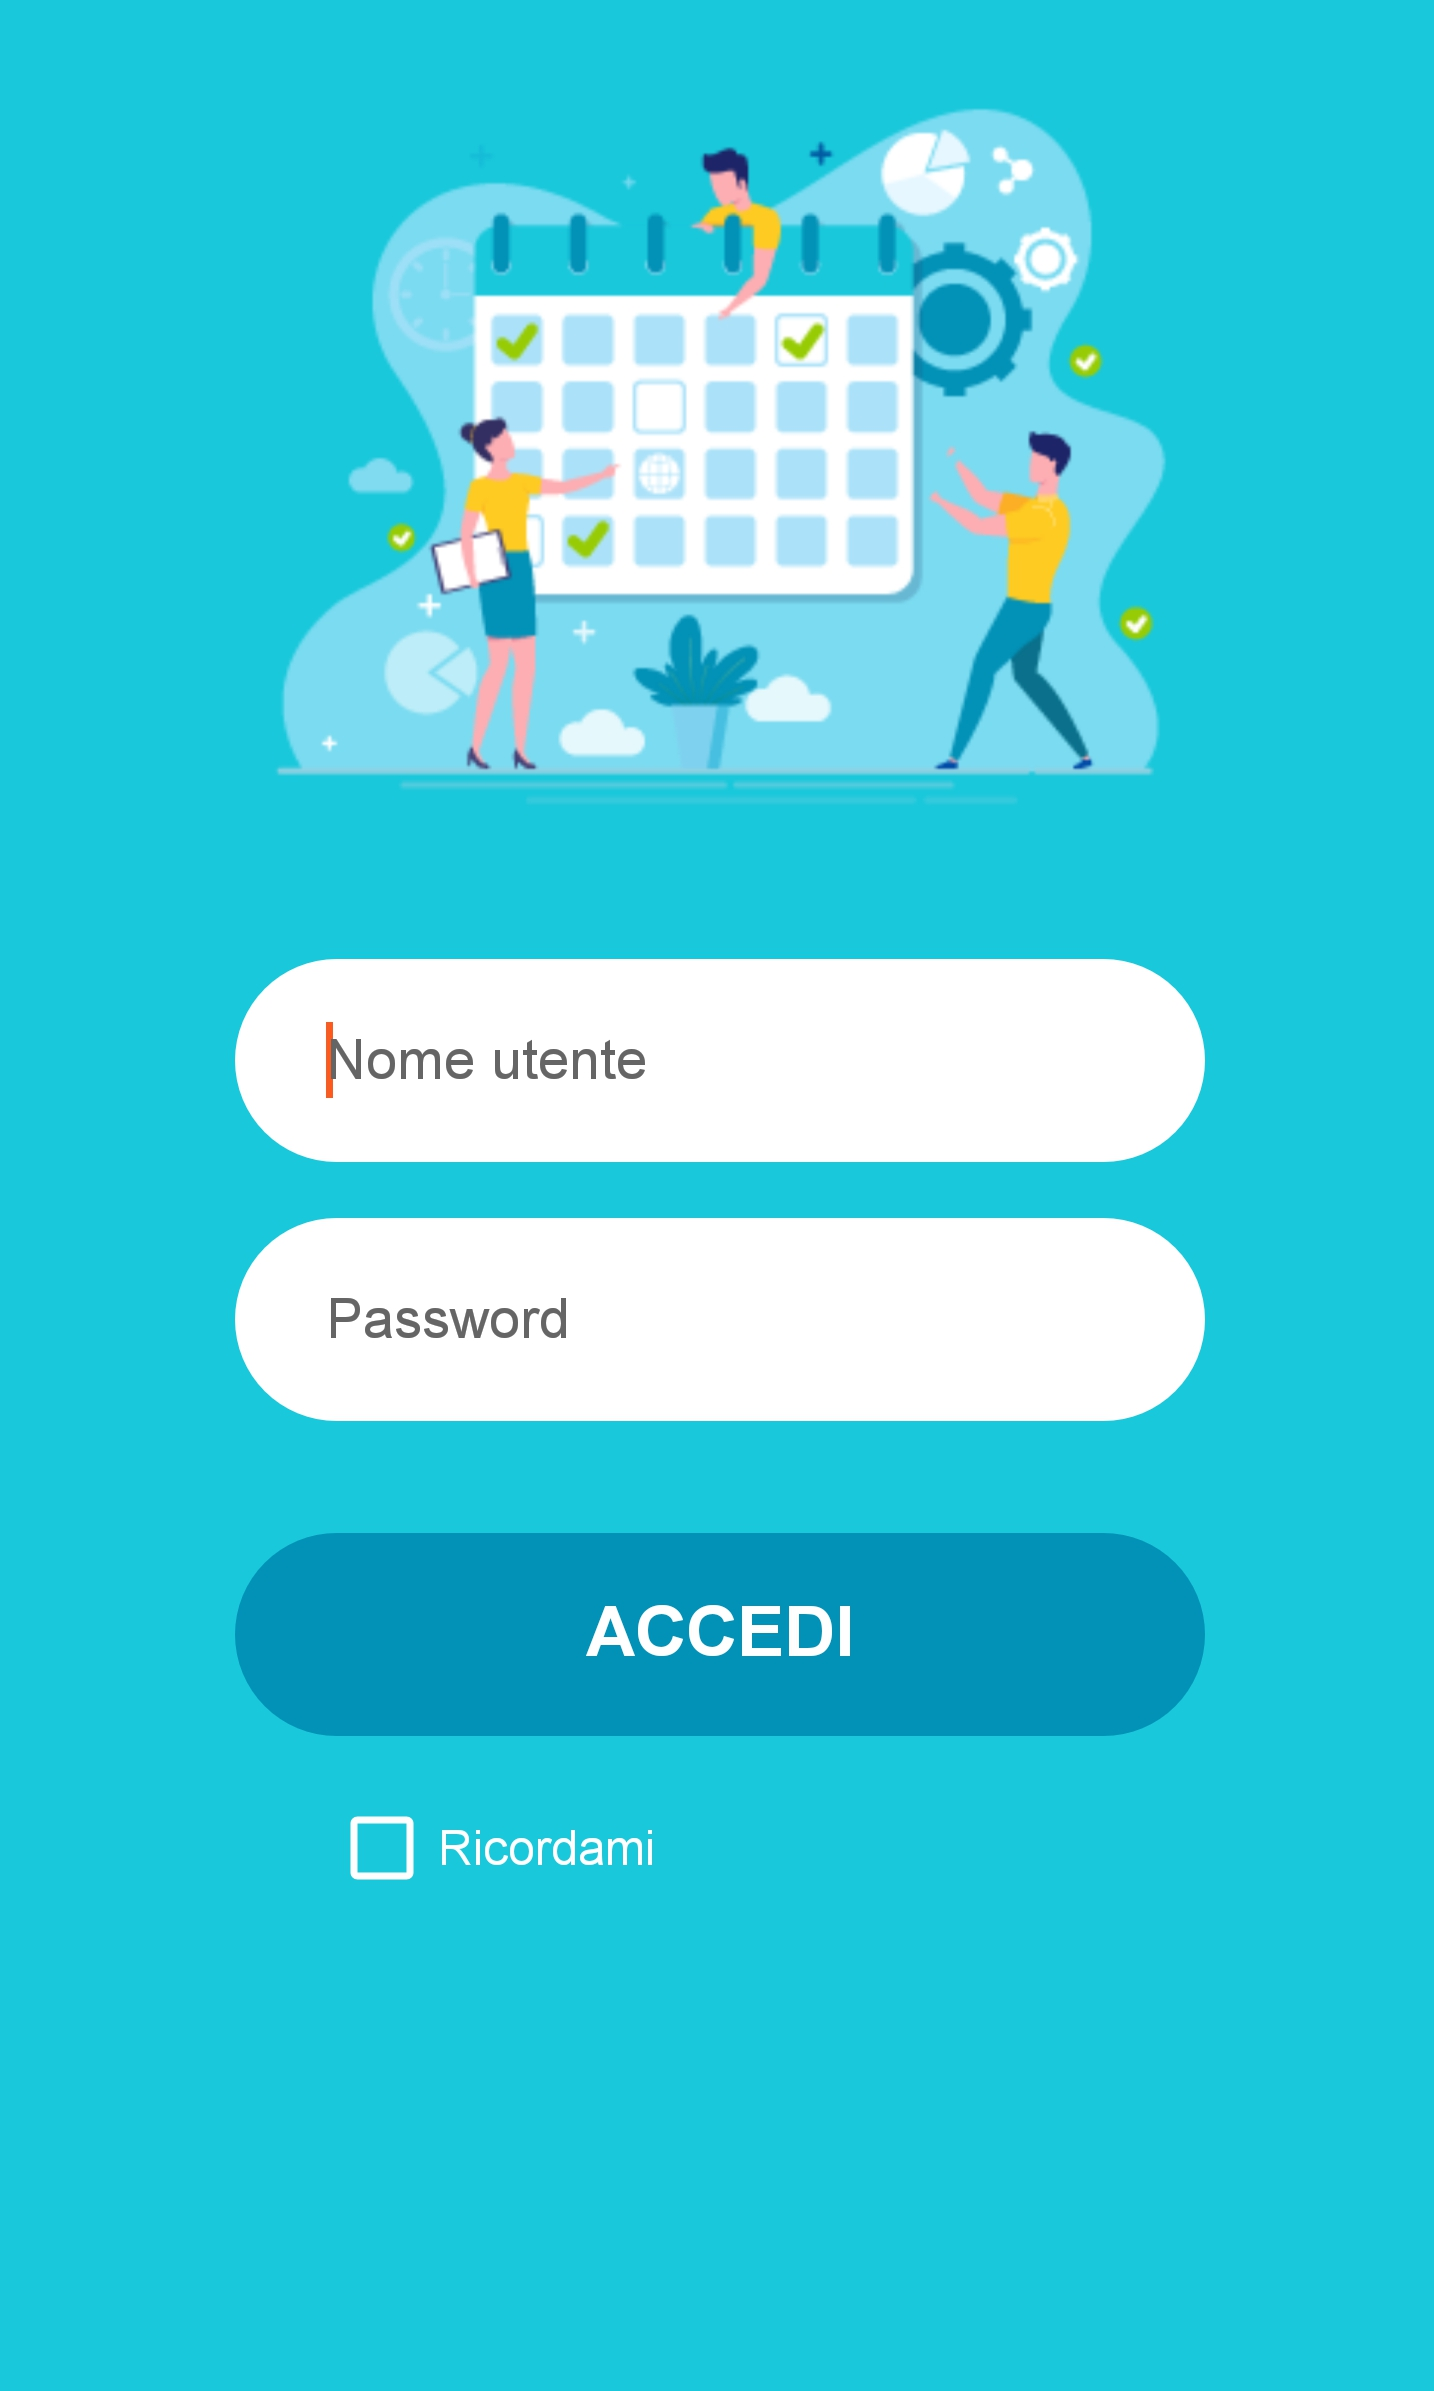
\includegraphics[width=0.3\linewidth]{immagini/login}
	\caption{}
\end{figure}
\newpage
Per rendere più veloce l'utilizzo dell'applicazione si è deciso di introdurre nella schermata di login l'opzione ricordarmi, in modo tale che l'utente dovrà inserire le credenziali solamente al primo accesso. Successivamente se l'opzione ricordami è spuntata, la schermata di login non verrà più mostrata, ma l'applicazione si avvierà effettuando l'accesso automaticamente mostrando come schermata principale il calendario con mese e giorno attuali già selezionati, permettendo così all'utente di concentrarsi al meglio sulle operazioni da svolgere e non ricordare ogni volta le proprie credenziali. Se l'accesso fallisce, viene mostrata nuovamente la schermata di login in modo tale che l'utente possa rieseguire l'accesso. Nell'applicazione non è prevista una schermata di registrazione in quanto l'azienda prevede di inserire manualmente, tramite il gestionale dei dipendenti una nuova persona assunta e comunicargli poi numero di matricola associato e password per accedere al sistema.

\section{Evaluation}
L'ultima fase del processo di progettazione delle interfacce consiste nel valutare il design realizzato e verificare che soddisfi il cliente. I test di valutazione sono cominciati prima che le intere schermate fossero realizzate in modo definitivo dagli sviluppatori. La progettazione e il testing sono due processi che vengono eseguiti contemporaneamente. É importante: ideare la schermata, testarla, modificarla e, quando si raggiunge l'obiettivo finale, implementarla. Per testare le varie schermate è stato utilizzato \textit{il test dei cinque secondi} che ha permesso di comprendere quali informazioni apprendono gli utenti e quale impressione ottengono entro i primi cinque secondi dalla visualizzazione di una schermata. Questo test viene utilizzato per verificare che un'interfaccia comunichi in modo efficace e chiaro il messaggio per cui è stata realizzata. Perchè cinque secondi? Da numerosi studi effettuati è emerso che cinque secondi è abbastanza tempo per coinvolgere un utente e comunicargli un messaggio in modo efficace, per questo è importante avere un design che comunichi in modo chiaro, quali sono le informazioni principali.
Il test dei cinque secondi è stato eseguito su 4 persone di età compresa tra i 27 e 30 anni, le quali hanno evidenziato le seguenti criticità:
\begin{itemize}
	\item I comandi per cancellare gli elementi di una lista non erano sufficientemente chiari e diversi tra le varie schermate, alcuni cercavano di eliminare un elemento tramite swipe, altri premendovi a lungo, perciò il team di sviluppo ha deciso di implementare
	entrambi i modi, adattando così l'applicazione alle abitudini degli utenti.
	\item Durante il salvataggio non veniva fornito nessun feedback visivo sull'esito dell'operazione. È stato introdotto un pannello che mostra un'icona verde o rossa in base allo stato dell'operazione eseguita.
\end{itemize}
In seguito, grazie ai test effettuati sugli utenti, le schermate sono state modificate e infine nuovamente fatte testare. Gli utenti dopo le modifiche non hanno evidenziato ulteriori criticità.\\
Di una notevole importanza c'è da evidenziare che indipendentemente dalla tecnica utilizzata per testare le varie schermate, il risultato finale comunque dipenderà dalla tipologia di utenti coinvolti, come dimostrano numerosi studi svolti. Ad esempio c'è un notevole divario tra gli studenti e le persone più anziane che utilizzano la stessa applicazione.\cite{Test}


\chapter{Dettagli implementativi}
In questo capitolo verranno presentati gli aspetti più tecnici riguardanti l'implementazione dell'applicazione mettendo in risalto i pattern architetturali, le tecnologie adottate e il loro utilizzo. 
\section{I pattern architetturali}
Prima di implementare il software, sono stati esaminati i pattern architetturali più comuni nell'ambito mobile, cercando di evidenziarne vantaggi e svantaggi di ognuno, permettendomi di comprendere il loro funzionamento e implementare il modello architetturale che meglio si adattava all'applicazione.
\subsection{Cenni teorici}
\begin{center}
	\textit{L’architettura software è l’organizzazione di base di un sistema, espressa dalle
	sue componenti, dalle relazioni tra di loro e con l’ambiente, e dai principi che ne
	guidano il progetto e l’evoluzione.} [IEEE/ANSI 1471–2000]\cite{architettura}
\end{center}
Lo scopo dell'architettura è quello di scomporre il sistema in vari sottosistemi. La realizzazione di componenti distinti è meno complessa rispetto a realizzare tutto il sistema in modo monolitico. Ridurre la complessità permette anche di migliorare le caratteristiche finali e la qualità del prodotto realizzato. L'utilizzo di un'architettura software è molto importante in progetti di medie/grandi dimensioni perchè permette di strutturare il sistema in modo tale che possieda determinate caratteristiche software. La scelta di quale architettura utilizzare viene influenzata dalle parti che compongono il sistema, dagli stakeholders e dall'esperienza dei programmatori. Questi fattori a loro volta influenzano parametri importanti come performance, safety, availability, maintainability e security. Durante la realizzazione è necessario compiere delle scelte considerando alcuni parametri più importanti di altri. La scelta viene effettuata in base al dominio di utilizzo e alle caratteristiche che il sistema finale dovrà possedere. Ad esempio, in un prodotto utilizzato nell'ambito medico si prediligono parametri come: safety e availability, mentre in un prodotto utilizzato dalle banche si prediligono parametri come security, maintainability, availability.
Un'architettura viene rappresentata mediante un diagramma a blocchi che illustra in modo astratto una vista della struttura del sistema. Un'architettura può essere conforme a modelli o stili architetturali generici, ognuno rappresenta una prospettiva differente del modello che si vuole realizzare.
\begin{enumerate}
	\item Struttura statica: il modello mostra la maggior parte dei componenti di un sistema
	\item Processo dinamico: il modello mostra la struttura del processo del sistema
	\item Modello a interfaccia: definisce i sottosistemi dell’interfaccia
	\item Modello entità relazione (ER): mostra le relazioni tra i vari sottosistemi
	\item Modello distribuito: mostra come sono distribuiti i vari sottosistemi nelle varie macchine
\end{enumerate}
L'utilizzo di architetture nell'ambito mobile è molto comune in quanto permette di suddividere il codice in vari sottosistemi. Solitamente, un sistema si occupa di gestire le viste e raccogliere gli input dell'utente, un altro sistema si occupa di accedere e manipolare i dati e, infine, un sistema coordina i vari sottosistemi. Nello sviluppo mobile Android gli sviluppatori non sono vincolati ad utilizzare particolari architetture, la qualità finale del software realizzato dipenderà esclusivamente dall'esperienza dello sviluppatore a differenza dello sviluppo mobile iOS in cui gli sviluppatori sono tenuti a utilizzare un'architettura Model View Controller.\\
Di seguito vengono descritti i modelli di architetture più comunemente utilizzati nello sviluppo di applicazioni mobile.
%http://didawiki.di.unipi.it/lib/exe/fetch.php/informatica/is-a/architetture14.pdf
\subsection{MVC (Model View Controller)}
\begin{figure}[H]
	\centering
	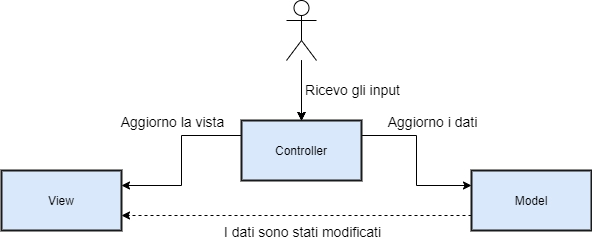
\includegraphics[width=0.7\linewidth]{immagini/mvc}
	\caption{}
	\label{fig:mvc}
\end{figure}
Il pattern architetturale MVC è basato sulla separazione dei componenti in tre moduli. La figura sopra riportata rappresenta un'architettura model view controller con i tre moduli principali e le loro interazioni. I tre componenti che la caratterizzano sono: 
\begin{enumerate}
	\item Il \textbf{M}odel: si occupa di fornire all'applicazione i metodi per recuperare, accedere e manipolare i dati
	\item La \textbf{V}iew: ha lo scopo di visualizzare i dati contenuti nel modello tramite gli elementi grafici disegnati nelle schermate. In Android una vista è rappresentata da un layout in formato XML che contiene i componenti base come: Button, TextView, Spinner, ecc...
	\item Il \textbf{C}ontroller: ha lo scopo di ricevere e interpretare i comandi utente, notificare al modello quali azioni eseguire sui dati e aggiornare la vista. In Android solitamente il controller viene rappresentato tramite un fragment o un'activity
\end{enumerate}
\newpage
\noindent
\textbf{Vantaggi}\\\\
Il modello MVC ha il vantaggio di suddividere le varie componenti che caratterizzano un'applicazione in modo indipendente tra loro, permettendo così a più persone con competenze diverse di collaborare insieme. Inoltre il model, non avendo dipendenze con il framework Android è possibile testarlo in isolamento, realizzando degli unit test che vengono eseguiti sulla Java Virtual Machine (JVM). Le viste sono isolate dall'implementazione dei dati e non conoscono la business logic, permettendo così di essere indipendenti dal modello e quindi facilmente testabili.\\
\\\textbf{Svantaggi}\\\\
Lo svantaggio principale dell'architettura MVC è che la vista viene utilizzata sia dal controller che dal modello, ed un'eventuale modifica di alcuni elementi nella vista potrebbe richiedere di modificare altri componenti che dipendono da essa, rendendo così questo modello rigido alle modifiche.
\subsection{MVP (Model View Presenter)}
\begin{figure}[H]
	\centering
	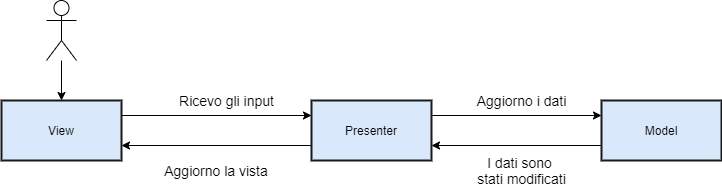
\includegraphics[width=0.7\linewidth]{immagini/mvp}
	\caption{}
	\label{fig:mvc}
\end{figure}
L'architettura MVP illustrata nella figura sopra riportata è composta da tre componenti principali:
\begin{enumerate}
	\item Il \textbf{M}odel: contiene la logica di business e i metodi per manipolare i dati %di come essi devono interagire tra loro
	\item La \textbf{V}iew: implementa un'interfaccia che espone i componenti al presenter, il quale utilizza questi metodi per manipolare la vista. In Android generalmente una vista è implementata da un fragment o da un'activity la quale in questo modello espone, mediante un'interfaccia, dei metodi come: updateData(), dropView(), hideButton()
	\item Il \textbf{P}resenter: è il componente principale che caratterizza l'architettura MVP. Svolge la funzione di mediatore tra la vista e il modello. Tramite l'interfaccia raccoglie gli input che l'utente fornisce, notifica al modello le operazioni da svolgere sui dati. Quest'ultimo invia le modifiche al presenter, che provvederà ad aggiornare la vista. C'è una relazione uno a uno tra la vista e il presenter, quindi ogni vista ne avrà associato uno, che interpreterà gli input dell'utente
\end{enumerate}
\textbf{Vantaggi}\\\\
L'architettura MVP permette di avere una maggiore testabilità del codice, in quanto il modello e il presenter non possiedono dipendenze dall'architettura Android, inoltre la vista è separata dal modello, il quale non ha dipendenze dirette con essa.
\\
\\\textbf{Svantaggi}\\\\
Strutturare un software che utilizzi un'architettura MVP richiede una notevole quantità di tempo e la scrittura di numerose righe di codice per implementarla, richiedendo una certa esperienza agli sviluppatori. Un altro svantaggio che ne deriva dal suo utilizzo è che il presenter può essere composto da numerosi metodi, e quindi è spesso soggetto a modifiche.
\subsection{MVVM (Model View ViewModel)}

\begin{figure}[H]
	\centering
	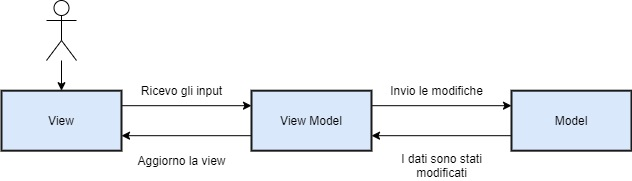
\includegraphics[width=0.7\linewidth]{immagini/mvvm}
	\caption{}
	\label{fig:mvc}
\end{figure}
Il pattern architetturale MVVM è composto da tre componenti principali:
\begin{enumerate}
	\item Il \textbf{M}odel: contiene i metodi per accedere e manipolare i dati %Solitamente l'accesso comporta l'utilizzo di web service o altre forme che permettono di ottenere i dati da una fonte.
	\item La \textbf{V}iew: si occupa di catturare gli input dell'utente e passarli al ViewModel. La differenza sostanziale del modello rispetto al MVP è come i dati vengono aggiornati nella vista. Nei pattern architetturali descritti precedentemente si utilizzavano metodi che venivano chiamati dai vari sistemi i quali si occupavano di aggiornare la vista. Nel modello MVVM viene utilizzata l'associazione dei dati (binding) tra vista e ViewModel, che permette un'associazione diretta tra i due moduli e, quindi, non è necessario implementare metodi per mettere in comunicazione i due moduli. Nel modello MVVM esiste una relazione di tipo molti-a-uno tra il ViewModel e la vista, più viste possono utilizzare gli stessi dati e la stessa logica contenuta in un singolo ViewModel
	\item Il \textbf{V}iew\textbf{M}odel: è il componente che permette di mettere in comunicazione la vista con il modello dei dati. % creando un canale di comunicazione unidirezionale con la vista.
	Gli scopi principali del ViewModel sono: esporre i dati, lo stato dell'applicazione ed eventuali messaggi di errore, validare l'input, eseguire tramite i metodi forniti dal modello le modifiche sui dati e infine eseguire le operazioni sulle viste per riflettere eventuali aggiornamenti dei dati. Il ViewModel non ha un riferimento con la vista ma quest'ultima viene collegata ad esso quando necessario % inviandogli gli input, che successivamente verranno elaborati ed eseguita l'operazione.

\end{enumerate}
\textbf{Vantaggi}\\\\
L’utilizzo dell'architettura MVVM permette di ridurre il numero delle linee di codice che implementano una vista. L'utilizzo del data-binding permette di non dover aggiornare manualmente una vista quando i dati vengono modificati.
\\
\\\textbf{Svantaggi}\\\\
Il problema principale di questo modello è che nelle applicazioni di grandi dimensioni il ViewModel può contenere molte linee di codice per gestire la business logic e la validazione dei dati, rendendo eventuali modifiche complesse. Un ViewModel di grandi dimensioni viola il principio di single responsability previsto dai principi SOLID\cite{solid}, rendendo il codice poco manutenibile. L'utilizzo del data-binding rende difficile il debug in quanto non permette di impostare dei punti di controllo durante l'esecuzione.
\\\\
%\subsection{MVI (Model View Intent)} nel caso vuoi aggiungere roba
Di seguito viene riportata una tabella che mette a confronto le varie architetture descritte, evidenziandone vantaggi e svantaggi.
\begin{table}[h]
	\centering
	
	\begin{tabular}{|l||ccc|}
		\hline
		\rule{0pt}{25pt} PATTERN &
		\multicolumn{1}{l|}{\begin{tabular}[c]{@{}l@{}}Dipendenze dal\\ framework Android\end{tabular}} &
		\multicolumn{1}{l|}{\begin{tabular}[c]{@{}l@{}}Complessità dei\\ file XML\end{tabular}} &
		\multicolumn{1}{l|}{\begin{tabular}[c]{@{}l@{}}Facilità\\ nel testing\end{tabular}} \\ \hline\hline
	%	\multicolumn{1}{l|}{Modularità} \\ \hline\hline
		\rule{0pt}{25pt} MVC  & {\color[HTML]{CB0000} Alta}  & {\color[HTML]{009901} Bassa} & {\color[HTML]{CB0000} Difficile} \\ \hline
		\rule{0pt}{25pt} MVP  & {\color[HTML]{009901} Bassa} & {\color[HTML]{009901} Bassa} & {\color[HTML]{009901} Buona}   \\ \hline
		\rule{0pt}{25pt} MVVM & {\color[HTML]{009901} Bassa} & {\color[HTML]{FFC702} Media} & {\color[HTML]{009901} Ottima}  \\ \hline
	\end{tabular}
	
%	\caption{Comparazione d delle varie architetture}
\end{table}
\newpage
\subsection{Considerazioni}
Le architetture descritte presentano diversi vantaggi e svantaggi, ma non ce n'è una migliore delle altre. Il loro obiettivo comune è quello di creare una separazione tra i vari elementi che compongono un'applicazione. 
L'utilizzo di un'architettura permette agli sviluppatori di mantenere il codice ben strutturato e organizzato. La scelta di quale utilizzare dipende dal tipo di applicazione che si vuole sviluppare e dalla sua dimensione. L'utilizzo di modelli complessi in progetti di piccole dimensioni composti da poche viste e funzionalità, comporta l'introduzione di una complessità non necessaria, complicando la realizzazione del prodotto. Tuttavia in un'applicazione di medie/grandi dimensioni, che utilizza numerose schermate e dati provenienti da diverse sorgenti, è consigliato l'utilizzo di un'architettura, perchè permette di organizzare il software e offre diverse qualità.\\
Nello sviluppo dell'applicazione è stato deciso di utilizzare un'architettura MVVM in quanto, recentemente, Android ha rilasciato una libreria (descritta nella successiva sezione), che permette di realizzare in modo semplice e veloce un'architettura MVVM. Il rilascio di questa libreria ha fatto si che, per la prima volta, Google incoraggi gli sviluppatori a strutturare le proprie applicazioni secondo un modello standard. Un altro fattore importante che ne ha determinato la scelta è stata l'esperienza pregressa nell'utilizzo di questo pattern architetturale da parte del team di sviluppo.

%https://android.jlelse.eu/why-to-choose-mvvm-over-mvp-android-architecture-33c0f2de55163
\section{Android Architecture Components}
Nel 2017 Google ha introdotto un insieme di librerie chiamate \textit{Android Architecture Components}, le quali permettono di implementare un'architettura software che renda le applicazioni robuste, testabili e facilmente manutenibili. %L'introduzione di queste librerie ha cambiato il modo con cui gli sviluppatori approcciano la realizzazione di un'applicazione android. Con l'introduzione di questi componenti Google consiglia un'architettura di tipo mvvm per le proprie applicazioni, questo non era mai stato fatto prima nel mondo android. 
Google ha deciso di consigliare un'architettura perchè sempre di più oggi le applicazioni sono composte da molteplici compiti, ad esempio: gestire le viste, i dati, le interazioni con gli utenti e il collegamento ad internet.\\

Con l'introduzione di questi componenti Google si pone anche l'obiettivo di risolvere il problema della persistenza dei dati all'interno di un'applicazione.\\
Android è un sistema operativo che nasce con lo scopo di utilizzare poche risorse hardware, per questo ottimizza la gestione della memoria distruggendo i componenti non più necessari, con la conseguente perdita di informazioni. Ogni componente inoltre è caratterizzato da un proprio ciclo di vita, il quale viene controllato dal sistema in base agli eventi generati dall'utente. Tramite delle callback gli sviluppatori rilevano queste interazioni e pianificano le reazioni. L'introduzione delle librerie e l'utilizzo dell'architettura proposta hanno portato due principali vantaggi nello sviluppo di un'applicazione:

\begin{comment}

Ogni componen componente realizzato ha un proprio ciclo di vita all'interno dell'applicazione e viene contronllato dal sistema in base agli eventi e al comportamento dell'utente. Gli sviluppatori tramite delle callback rilevano le interazioni utente e pianificano le reazioni. Durante l'esecuzione di un'applicazione molteplici componenti collaborano tra loro in diversi momenti.Android è framework che nasce con lo scopo di utilizzare poche risorse hardware per questo cerca di utilizzare al meglio la propria memoria distruggendo i componenti non più necessari con la conseguenza perdita di informazione. Questa è una tematica molto importante e determina il ruolo particolarmente critico che la persistenza dei dati assume in Android.\\

I principi su cui si basa l'architettura proposta da google sono:
	contenuto...
\end{comment}
\begin{enumerate}[label=\arabic*)]
	\item La \textit{Separazione delle competenze:} ogni componente dell'applicazione deve essere indipendente dagli altri e implementare solo le proprie competenze. Gli sviluppatori dovrebbero evitare di accumulare troppe funzionalità in un'activity o fragment, in quanto il sistema operativo può distruggerle in qualsiasi momento in base alle interazioni dell'utente o a causa di memoria insufficiente. Per fornire un'esperienza utente fluida e reattiva è consigliato ridurre al minimo le dipendenze da fragment o activity.
	\item \textit{L'utilizzo di un modello per gestire la UI} è una pratica che viene introdotta con le librerie contenute negli Android Architecture Components in particolare con l'utilizzo dei ViewModel. Questo componente permette di gestire in modo persistente i dati dell'applicazione separandoli dagli altri elementi che caratterizzano l'interfaccia utente, rimanendo indipendenti dal ciclo di vita dell'applicazione.
\end{enumerate}
Di seguito viene raffigurato il modello dell'architettura presentata da Google, che evidenzia i moduli e le relazioni che la caratterizzano.
\newpage
\begin{multicols}{2}
	\begin{figure}[H]
		\centering
		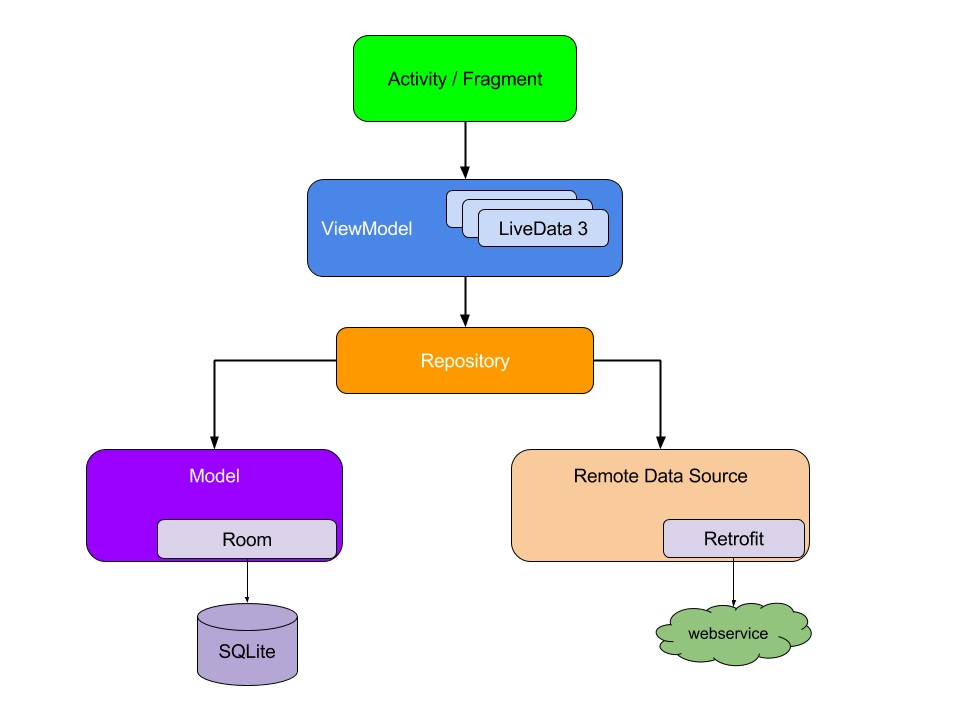
\includegraphics[width=1.1\linewidth]{immagini/final-architecture}
		\caption{}
		\label{}
	\end{figure}
	\begin{figure}[H]
		\centering
		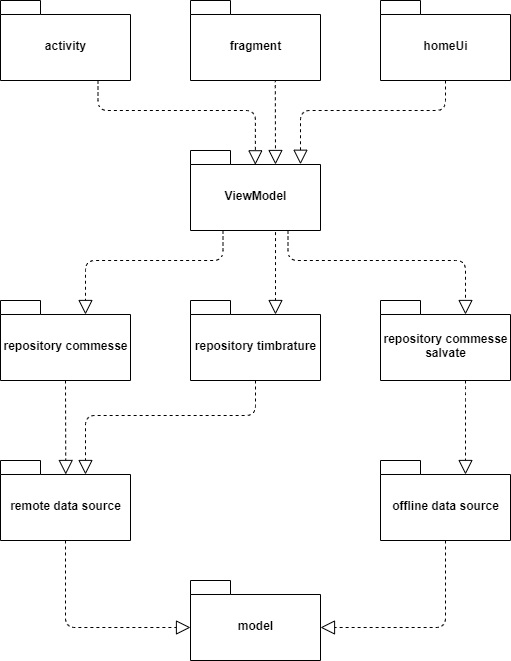
\includegraphics[width=0.8\linewidth]{immagini/architecture}
		\caption{}
		\label{Modello realizzato per definire l'architettura finale}
	\end{figure}
\end{multicols}
L'applicazione finale è stata implementata seguendo il modello architetturale sopra riportato che, come si può evincere dalle due immagini, aderisce alla struttura proposta dalle guide ufficiali. Dal modello si può notare come ogni componente dipenda solo dai componenti ad un livello al di sotto di esso, rendendo il testing facile. Questa struttura insieme all'utilizzo dei LiveData permette di mantenere i dati separati dal ciclo di vita dell'applicazione e separare le competenze in vari moduli. L'utilizzo dei LiveData permette di fornire all'utente sempre gli ultimi aggiornamenti infatti, se i dati non rappresentano l'attuale situazione, i repository scaricheranno i dati dal database in modo del tutto trasparente all'utente. I dati ottenuti dalle sorgenti remote vengono salvati all'interno di un database SQLite, che viene utilizzato come una cache per i dati. Anche in assenza di una connessione ad internet sarà possibile utilizzare comunque l'applicazione. Eventuali modifiche eseguite offline verranno riportate anche sul database online quando la connessione tornerà disponibile, viceversa l'applicazione scaricherà eventuali modifiche effettuate nel database remoto. Questa struttura ha il forte vantaggio di mostrare sempre i dati più aggiornati senza che l'utente svolga nessuna azione di aggiornamento.\\
Uno degli elementi centrali offerti dagli Android Architecture Components è il ViewModel, questo componente ha lo scopo principale di gestire i dati dell'interfaccia utente che vengono forniti tramite i repository ad una o più Activity o Fragment. Il ViewModel non conosce com'è costituita l'interfaccia utente e quindi non è influenzato da essa, perciò l'eventuale distruzione o sospensione di una vista non farà perdere i dati che la caratterizzano. Se invece i dati fossero stati scaricati e manipolati direttamente all'interno di una vista, quando questa viene distrutta i dati andranno persi. Il ViewModel viene valorizzato utilizzando oggetti LiveData che sopravvivono al ciclo di vita e popoleranno l'interfaccia utente. Per ottenere i dati vengono utilizzati dei repository. Questi moduli hanno lo scopo di fornire delle Application Programming Interface API, che espongono dei metodi permettendo al ViewModel di ottenere i dati senza conoscere quale sia la sorgente e il modo di ottenerli. Ad esempio, non conosce se i dati sono ottenuti da un database remoto tramite web service oppure è stato interrogato un database locale.\\
 É possibile vedere i repository come dei mediatori tra diverse sorgenti di dati, che offrono servizi di cache, web e di persistenza. Nell'applicazione sviluppata sono stati realizzati tre repository, in modo da suddividere le APIs in tre moduli indipendenti tra loro. I repository delle commesse e timbrature utilizzano un modulo per eseguire delle chiamate rest ad un servizio web, mentre il repository delle commesse salvate utilizza un database SQLite locale per mantenere una copia di alcune commesse precedentemente scaricate.
\\Di seguito viene rappresentato il codice di un ViewModel che ha lo scopo di autenticare un utente mediante lo username e la password.
\lstinputlisting{./codici/viewModelLogin.java}
Il repository degli utenti si occupa di eseguire delle chiamate a un web service che permette di verificare le credenziali inserite. Di seguito viene riportata l'implementazione.
\lstinputlisting{./codici/repositoryUser.java}
% Dobbideveloper.android.com/jetpack/docs/guide
% https://www.html.it/pag/69822/viewmodel-e-livedata/ 
%stavo leggendo questi articoli continua da qui
%volevo inserire degli esempi di codice, e continuare fino a riempire la pagina, mostro come si inserisce un ViewModel in un'activity e come esso è implementato mostrando un'implementazione di base poi mostro i vieModel implementati
\subsection{LiveData}
Per gestire il recupero dei dati provenienti da diverse fonti, sono stati utilizzati i LiveData. Questo modulo contenuto sempre all'interno degli Android Architecture Components aderisce al pattern \textit{observable} \cite{observer}, il quale permette di rilevare istantaneamente i cambiamenti che vengono effettuati ai dati, notificando agli oggetti (solitamente le viste), che registrano un osservatore, i cambiamenti apportati. La caratteristica principale che ha reso particolarmente utili i LiveData all'interno del progetto è che il modello conosce il ciclo di vita dell'applicazione, portando i numerosi vantaggi di seguito elencati.
\begin{enumerate}
	\item Assicurano che l'interfaccia utente mostri i dati più recenti. Grazie al pattern observer, quando avviene una modifica ai dati, queste vengono immediatamente riflesse nella vista, attivando l'osservatore che essa ha registrato.
	\item Nessun arresto a causa di attività in background. Quando un'activity o fragment è nello stato di sospensione, un eventuale aggiornamento dei LiveData ad essi associati non viene notificato perchè le viste sono in uno stato inattivo.
	\item Non è più necessario gestire manualmente il ciclo di vita dell'applicazione, infatti i componenti dell'UI registrano un osservatore sui dati che gli interessano e i LiveData decidono quando notificare le modifiche o rimuovere un osservatore da una vista.
	\item Non è necessario gestire la rotazione dello schermo. Quando un dispositivo viene ruotato il fragment o activity viene ricreato riscaricando i dati. Grazie ai LiveData non è più necessario gestire manualmente la rotazione, quando lo smartphone viene ruotato, automaticamente il LiveData invia i dati più aggiornati che possiede.
	\item Condivisione dei dati con più viste. I LiveData aderiscono anche al pattern singleton\cite{singleton}, creando una sola istanza dell’oggetto, perciò più viste potranno registrare un osservatore unico per ogni LiveData, quando i dati verranno modificati, verrà notificato a tutte le viste (in base al loro stato) che i dati sono cambiati, le quali aggiorneranno il proprio stato.

\end{enumerate}
Di seguito viene riportato il codice che mostra come vengono utilizzati i LiveData per scaricare in modo asincrono una lista che contiene i giorni di un mese. Per il download vengono utilizzati dei web service descritti nella successiva sezione.
\lstinputlisting{./codici/livedata.java}
Il codice della vista riportato di seguito mostra l'osservatore registrato su un LiveData che fornisce la lista dei giorni. Il funzionamento di questo metodo è quello di interrogare tramite il ViewModel il repository per ottenere i dati. Quest'ultimo, deciderà in base allo stato attuale dell'applicazione e dei dati se scaricarli o fornirli dal database locale. Successivamente scriverà i dati nell'oggetto incapsulato, in questo caso una lista di giorni. A tutte le viste che gli osservano verrà notificato un aggiornamento e chiamato il metodo onChange. Le viste, a loro volta, aggiorneranno i propri elementi mostrando i nuovi dati all'utente.
\\
\lstinputlisting{./codici/vistaLiveData.java}
Per manipolare un oggetto di tipo LiveData è possibile utilizzare la libreria RxJava che, tramite la programmazione reattiva, permette di eseguire operazioni su flussi di eventi. Nell'applicazione, i flussi di dati gestiti derivano dalle chiamate effettuate dal repository ai web service.

%
%MOSTRA DEGLI ESEMPI DEL CODICE
%usando gli android componentes per ottenere i dati da internet gli ho inserite dentro i view model così loro gestiscono in automatico il ciclo di vita delle viste
%
\subsection{Room}
%https://www.html.it/pag/71033/room-orm-su-sqlite/
%teoria
%https://developer.android.com/training/data-storage/room/index.html
Uno dei requisiti dell'applicazione riportava la necessità di salvare in locale alcune commesse, in modo tale che l'utente possa recuperare velocemente gli ordini ai quali lavora più di frequente. Per implementare il salvataggio è stata utilizzata la libreria Room\cite{Room} disponibile all'interno degli Android Architecture Components e caratterizzata da un approccio Object-Relational Mapping (ORM) che consiste nel fornire, mediante un'interfaccia, tutti i servizi necessari per comunicare con il servizio di persistenza, astraendo al tempo stesso dalle caratteristiche tecniche dello specifico database utilizzato. 
Room utilizza come servizio di persistenza un database SQLite, Le componenti principali su cui si basa sono tre:
\begin{enumerate}
	\item 
	 Database Access Object (DAO): offre tramite dei metodi astratti le operazioni di creazione, lettura, aggiornamento e cancellazione. Tramite il DAO vengono definite le query che si vogliono eseguire nel database. In un'applicazione possono esistere diversi DAO.
	\item Entità: sono delle classi che rappresentano le tabelle del database. All'interno delle entità vengono definiti tramite delle variabili i campi previsti dallo schema ER che rappresenta la struttura del database.
	\item Database: rappresenta mediante una classe un'astrazione del database, tramite il DAO è possibile manipolare i dati in esso contenuti.
\end{enumerate}
Nella figura sottostante viene riportata una rappresentazione grafica dei componenti principali utilizzati in Room e come essi interagiscono tra di loro.
\begin{figure}[!h]
	\centering
	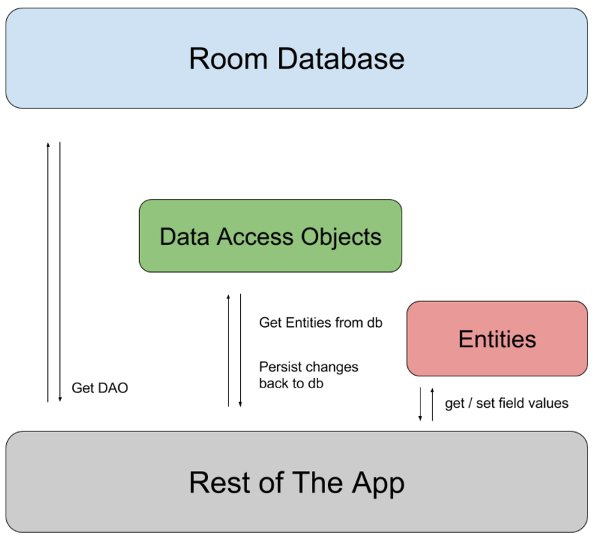
\includegraphics[width=0.4\linewidth]{immagini/room}
	\caption{}
	\label{fig:room}
\end{figure}
\newpage
Per realizzare i componenti viene utilizzato il framework Android Note. %\cite{annotazioni}.
Questo strumento permette agli sviluppatori di semplificare il codice nelle applicazioni e ridurre il numero di righe utilizzate comunemente per definire le strutture standard necessarie per realizzare un servizio di persistenza. Tramite l'annotazione @Database identifichiamo la classe che rappresenterà il nostro database, specificando la versione e le entità che lo compongono. Esso Contiene al suo interno un riferimento, tramite una classe astratta, al DAO.  Nel codice sotto riportato è possibile notare che la classe ha un riferimento interno ad una propria istanza, la quale fa si che il database aderisca al pattern singleton. Utilizzando \textit{databaseBuilder}, il database verrà salvato nella memoria locale in modo persistente. Quando l'applicazione verrà chiusa le informazioni salvate rimarranno in memoria. Nel caso si utilizzasse \textit{InMemorydatabaseBuilder}, quando l'applicazione verrà arrestata le informazioni salvate verranno cancellate perchè il database verrà salvato all'interno della memoria temporanea assegnata dal sistema operativo all'avvio. Nell'applicazione è stato implementato un servizio di persistenza per memorizzare alcune commesse. Questo è stato salvato nella memoria del telefono così che le informazioni siano sempre disponibili, anche in seguito a riavvi dell'applicazione.

\lstinputlisting{./codici/db.java}

Per definire una tabella è necessario utilizzare l'annotazione @Entity nella classe che la rappresenta. Tramite l'annotazione @PrimaryKey si identifica un attributo come chiave primaria, mentre le altre variabili rappresenteranno le restanti colonne della nostra tabella.
La classe di seguito riportata mostra l'entità \textit{Ordine}, la quale contiene un riferimento ad una commessa, mentre nella figura sotto riportata viene rappresentata la tabella implementata nel database.
\begin{figure}[h!]
	\centering
	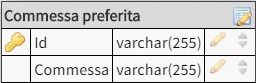
\includegraphics[width=0.3\linewidth]{immagini/db}
	\caption{}
	\label{fig:tabella_commessa}
\end{figure}
\lstinputlisting{./codici/entita.java}
Per definire le operazioni all'interno del DAO vengono utilizzate le annotazioni @Create, @Read, @Update, @Delete che implementano le comuni operazioni di creazione, lettura, aggiornamento e cancellazione. É possibile inoltre definire una query personalizzata utilizzando l'annotazione @Query e implementare il codice sql che la definisce. Di seguito viene riportata l'implementazione del DAO utilizzato per interagire con il database, oltre ad offrire le query standard ne viene definita una personalizzata che permette di ottenere il numero totale di ordini inseriti nel database. Non è necessario implementare i metodi all'interno del DAO, la loro implementazione avverrà in fase di compilazione da parte del compilatore.
\lstinputlisting{./codici/dao.java}
L'utilizzo della libreria Room e delle annotazioni ha permesso di implementare un semplice database SQLite, scrivendo molte meno linee di codice rispetto ad un'implementazione standard. Inoltre l'integrazione immediata con i LiveData ha permesso di ottenere tutti benefici che ne derivano dal loro utilizzo.
\section{Json Web Service}
Una parte importante del progetto è caratterizzata dall'interazione tra l'applicazione e i web service messi a disposizione dall'azienda che permettono di interagire con la base di dati. Tramite il protocollo Hypertext Transfer Protocol (HTTP/1.1)\cite{http} è possibile comunicare con il server, che a sua volta interroga il database e restituisce le risposte nel formato JavaScript Object Notation (JSON). Oggi questo formato è comunemente utilizzato per lo scambio di dati tra client e server. JSON nel tempo è stato standardizzato, l'ultimo standard è stato pubblicato nel 2017 come RFC 8259\cite{json}. I dati di base previsti dalla normativa sono i seguenti:
	\begin{enumerate}
		\item Numero: un numero decimale con segno più l'eventuale parte frazionaria. Può contenere anche la notazione esponenziale. Il tipo NaN non è previsto.
		\item Stringa: le stringhe devono contenere caratteri unicode e sono delimitate dalle doppie virgolette. Il carattere '/' è utilizzato come escape nel caso la stringa contenga caratteri speciali.
		\item Booleano: il dato booleano è rappresentato dal valore true o false.
		\item Lista: la lista è rappresentata da due parentesi quadre, quella aperta identifica l'inizio della lista, mentre la chiusa ne determina la fine. I valori contenuti nella lista vengono separati da una virgola.
		\item Oggetto: un oggetto viene rappresentato nel formato json con una coppia (attributo:valore), per ogni elemento che caratterizza l'oggetto avremo una coppia. Gli oggetti vengono delimitati da parentesi graffe, le virgole per separare ciascuna coppia, mentre i due punti vengono utilizzati per separare l'attributo dal proprio valore.
		\item null: il valore null identifica un valore vuoto.
	\end{enumerate}

\lstinputlisting[language=json,caption=Esempio di una lista contenente un oggetto,captionpos=b]{./codici/jsExample.json}	
I web service hanno permesso di mettere in comunicazione l'applicazione con il server che contiene i dati di ogni singolo dipendente e le informazioni relative ad ogni progetto. L'utilizzo della libreria OkHttp ha permesso di realizzare in modo efficiente e compatto le chiamate HTTP al server. I web service utilizzano diversi parametri previsti dal protocollo. Il metodo POST viene utilizzato per inviare i dati al server e comunicargli di creare o aggiornare dei dati nel database. Il metodo PUT viene utilizzato per inserire elementi all'interno del database. L'utilizzo di PUT è simile a POST ma idempotente, cioè è possibile eseguire più volte una chiamata PUT la quale produrrà in output sempre lo stesso risultato. Il metodo DELETE viene utilizzato per cancellare delle risorse e infine GET per ottenere i dati dal database.\\
Ottenuti i dati nel formato testuale, è stato necessario associarli agli oggetti Plain Old Java Object (POJO). Il nome denota un oggetto Java serializzabile, che non dipende da nessun framework, possiede un costruttore senza argomenti e consente l'accesso ai suoi attributi tramite i metodi \textit{getter} e \textit{setter}. La libreria Gson sviluppata da Google permette di trasformare dei dati in formato json in un oggetto POJO e viceversa, senza richiedere allo sviluppatore di implementare codice per eseguire la trasformazione. Le operazioni vengono eseguite all'interno di Android, utilizzando una classe apposita, che rappresenta un client web, il quale permette al repository di comunicare con il server e di ottenere gli oggetti necessari per poi eseguire le varie operazioni.\\
Per utilizzare i web service, è necessario che l'utente si identifichi al server fornendo le proprie credenziali. Se corrette viene assegnato un token generato dal server, che identificherà l'utente per tutte le successive chiamate.
Ogni volta che si effettua un'operazione è necessario inviare il token al server per verificare l'autenticità del messaggio. L'utilizzo del token, insieme al protocollo SSL\cite{rfc6101}, permette di implementare un livello di sicurezza nella comunicazione tra l'applicazione e il server, garantendo che i dati scambiati siano confidenziali. Ogni 10 minuti il token viene revocato ed è quindi necessario rieseguire il login. Per evitare all'utente di inserire le credenziali dopo 10 minuti di utilizzo, alla prima chiamata effettuata queste vengono salvate all'interno dell'applicazione, rieseguendo il login automaticamente nel caso in cui il token sia stato revocato. Alla chiusura dell'applicazione le credenziali vengono eliminate se l'utente non ha selezionato, in fase di login, l'opzione ricordami.\\Per evitare modifiche concorrenti tra l'applicazione web e mobile è stato implementato all'interno di ogni json un attributo denominato \textit{rowVersion}. Il database implementa una politica di blocco pessimistico garantendo l'accesso esclusivo ad una risorsa. Ogni volta che viene eseguita una modifica ad un oggetto, quest'ultimo viene restituito dai web service con i campi modificati dall'operazione eseguita e il valore del rowVersion incrementato. Se in un'altra sessione contemporaneamente un utente dovesse eseguire la stessa operazione e inviasse un oggetto con un valore del rowVersion vecchio, questa verrebbe rifiutata, perchè i dati sono già stati modificati da un'altra sessione.




\chapter{Verifica}
Il testing come tecnica di controllo ha il principale obiettivo di verificare la correttezza del software. Viene utilizzato comunemente per valutare fattori di qualità come ad esempio affidabilità, usabilità ed efficienza. La fase di verifica è molto importante. Permette di accertare che il software realizzato rispecchi i requisiti e le specifiche definite nella fase di analisi. Alla fine dello sviluppo di un sistema è possibile che funzioni correttamente, ma che, al tempo stesso, sia del tutto inutile perchè non soddisfa i requisiti proposti nella fase di analisi. La verifica svolta nel progetto ha previsto l'utilizzo di framework appositi per realizzazione di test automatici con lo scopo di verificare che la UI e UX realizzata funzionasse come previsto dalle specifiche. La verifica in questo caso è stata di tipo \textit{dinamico} collaudando l'applicazione con verifiche visive e strumentali, utilizzando il framework Espresso.
\section{Android Testing}

Nel sistema Android è possibile eseguire tre diverse tipologie di testing. Dall'immagine sotto riportata è possibile vedere come ogni tipologia di test permetta di aggiungere uno strato di maggiore affidabilità all'applicazione.
\newpage
\begin{figure}[!h]
	\centering
	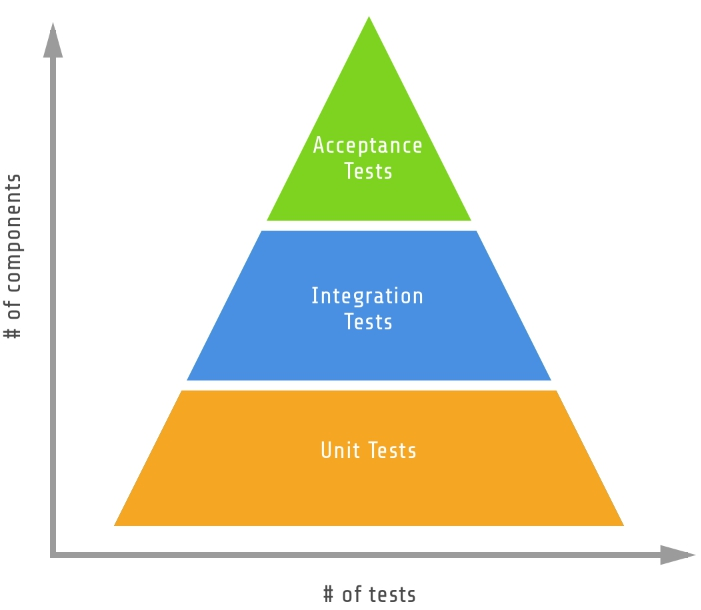
\includegraphics[width=0.5\linewidth]{immagini/testing_piramide}
	\caption{}
	\label{fig:testingpiramide}
\end{figure}
\begin{enumerate}
\item Lo \textit{unit test} viene solitamente utilizzato per testare codice java in isolamento, cioè eliminando le dipendenze dell'oggetto che vogliamo testare. Tramite l’utilizzo di librerie come Mockito è possibile simulare le dipendenze tramite degli oggetti chiamati mock. Solitamente il codice testato tramite unit testing sono i programmi che includono la business logic e la convalida dati. Questi test vengono eseguiti nella JVM, in quanto non avendo dipendenze dal framework Android, non è necessario avviare nessun device per eseguire i test, rendendo così i test più veloci in termini di tempo.

\item \textit{L’integration testing} viene utilizzato per verificare come i vari componenti interagiscono tra di loro. Tramite lo unit testing potrebbero essere eseguiti correttamente i test delle singole classi, ma quando queste collaborano tra loro per raggiungere un obiettivo comune, non è detto che il software funzioni come ci si aspetti. Tramite l’integration testing è possibile scoprire eventuali bug delle interfacce tra i vari moduli. In fase di sviluppo è importante realizzare test di integrazione, perché permettono agli sviluppatori di avere uno strato ulteriore di testing aumentando la copertura di codice testato, l’affidabilità dei test e del software finale. I test di integrazione sono importanti quando è necessario modificare il comportamento e/o le funzionalità offerte da uno o più moduli, perché permettono di verificare senza modificare i test, che il codice continui a funzionare in seguito alle modifiche.\\
In Android i test di integrazione vengono eseguiti su dispositivi reali o emulatori. Questo può essere uno svantaggio nel caso di software di medie o grandi dimensioni, che includono numerosi test, perchè l'esecuzione può richiedere una notevole quantità di tempo. %Per rendere i test più veloci è possibile questo problema viene utilizzato
É possibile rendere i test più veloci utilizzando il framework RoboElettric, che permette di eseguire test di integrazione tramite la JVM locale, senza quindi utilizzare dispositivi virtuali o emulati. Lo svantaggio del suo utilizzo, è che il framework non è gestito direttamente da Google, quindi è necessario attendere il rilascio di una nuova versione per eseguire i test nelle ultime versioni di Android. I test eseguiti con RoboElettric richiedono una maggiore quantità di tempo di esecuzione rispetto ai test di unità perché è necessario comunque avviare il framework Android. Utilizzare RoboElettric per tutti i test di integrazione non è un buon approccio. É consigliato suddividere i test in due tipologie: quelli che testano solo l’integrazione tra i moduli e non hanno dipendenze con il framework Android, quindi possono essere eseguiti nella JVM locale diminuendo così il tempo di testing. La seconda tipologia, sono i test che richiedono dipendenze di Android, in questo caso i test vengono eseguiti utilizzando RoboElettric.

\item \textit{UI Testing}. Per eseguire questa tipologia di test è necessario utilizzare un emulatore o un device fisico. I test simulano il comportamento e l’interazione che l’utente finale avrà con l’applicazione. L'approccio automatizzato consente di eseguire i test in modo rapido, affidabile e ripetibile.%secondo il paradigma Record&Playback.
\end{enumerate}

\begin{comment}
I test delle interfacce si suddividono in due categorie:
\begin{enumerate}
\item Test di ui/ux su singola app: questa tipologia ha lo scopo di verificare che l’ui e ux si comporti come previsto, quando un utente svolge un’attività specifica o immette un input in una vista si verifica che l’output dell’interfaccia utente corrisponda a quanto progettato. I framework di test della ui come Espresso consentono di simulare a livello di programmazione le azioni e interazioni che l’utente solitamente esegue nell’applicazione.

\item Test delle interfacce su più app: questa tipologia di test verifica il comportamento delle interazioni utente tra diverse app. Ad esempio, si potrebbe voler testare la condivisione tra un’informazione contenuta all’interno della propria app con una di terzi, oppure l’interazione tra la fotocamera di sistema e la propria app. Il framework più diffuso per eseguire questa tipologia di test è UiAutomator.
\end{enumerate}
Con espresso non è possibile testare le seguenti funzionalità:
Notifiche dell’applicazione
Sincronizzazione di informazioni con altre app
Navigazione in altre app che collaborano con la propria

Quando usare espresso o uiAutomator? Se lo scopo dei test è verificare che le interfacce funzionino in modo corretto nella nostra app allora espresso è una buona scelta, anche se limitata solo ai dispositivi android. Nel caso la nostra applicazione devo comunicare con altre applicazioni o gestire notifiche allora UiAutomator è lo strumento che ci permetterà di testare questa tipologia di interazioni.
Nelle ultime versioni di Espresso è stata introdotta l’estensione espresso-intent  che permette di simulare i dati che provengono da altre app, il suo utilizzo è simile a mockito, simulando quindi i dati che verrebbero fornite da app esterne.
	contenuto...
\end{comment}
\section{Android UI Testing Frameworks}

In questa sezione verranno discussi i framework più popolari in Android per eseguire UI testing. Le informazioni, apprese durante lo studio dei vari framework, hanno permesso di selezionare quello che meglio si adattava alla realizzazione di UI testing nell'applicazione finale. Tra i vari framework disponibili in commercio è stata prestata maggiore attenzione ad Espresso, Appium e Calabash in quanto sono quelli più ampiamente utilizzati.\cite{TestDiffusi}
%\\
%\underline{Descrivi cons'è un test black-box e white-box}
%\\
%\underline{http://jultika.oulu.fi/files/nbnfioulu-201706142676.pdf}
%\\
%\underline{https://webthesis.biblio.polito.it/6592/1/tesi.pdf}
\subsection{Cenni Teorici}
Il testing del software è una parte importante durante lo sviluppo di un prodotto. L'obiettivo principale dei test è affermare la qualità del sistema testandolo sistematicamente in modo controllato. Ci sono tre importanti tecniche per eseguire testing\cite{articleTesting}. In particolare i test definiti \textit{Black-Box Testing} hanno lo scopo di verificare che la business logic funzioni come progettato. In questo caso non si conosce come un singolo modulo è implementato, ci si limita a fornirgli degli input e verificare che l'output sia corretto. Un'altra tipologia di test è chiamata \textit{White-Box Testing} questa tecnica è simile ai black-box test, con la differenza che si ha un completa conoscenza del codice che implementa i vari moduli. La terza tipologia di testing è chiamata \textit{Grey-Box Testing} ed è la combinazione di White e Black box testing in cui si possiede una conoscenza parziale del codice. Questa tecnica di testing è utile principalmente nei test di integrazione.\\
Le tre tecniche descritte vengono comunemente utilizzate nei framework (descritti successivamente) per realizzare i test delle interfacce. %L'obiettivo principale è di verificare che le interfacce utente funzionino come definito nelle specifiche.
\subsection{Espresso e UIAutomator}
Espresso\cite{Espresso} è un framework open source rilasciato da Google che permette di realizzare testing strumentale nei device Android. Per implementare i test viene utilizzato Java o in alternativa Kotlin. I test realizzati vengono eseguiti su device fisici o virtuali, perchè per simulare l'interazione utente è necessario utilizzare il framework Android.\\
Espresso fornisce delle APIs semplici per scrivere i test e può essere utilizzato per testare le interfacce in device Android con API livello 10 fino alle ultime rilasciate.
La prima fase di un test consiste nel ricercare una vista, tramite gli attributi che la caratterizzano. Dopo averla selezionata, Espresso consente di eseguire delle azioni su di essa, simulando quindi le operazioni che l'utente svolgerebbe, come ad esempio, è possibile riempire campi di testo, analizzare gli output ed eseguire azioni. Il framework utilizza dei meccanismi di sincronizzazione, è quindi capace di verificare se una determinata vista è attiva o meno prima di eseguire un'operazione. Espresso permette di realizzare test che vengono eseguiti su una singola applicazione. Nel caso ci sia una condivisione di informazioni tra diverse applicazioni non sarà possibile eseguire test che verificano il passaggio di informazioni tra un'applicazione e l'altra. Google per permettere di eseguire UI testing in applicazioni che condividono informazioni con altre ha introdotto UIAutomator\cite{UIAutomator}. Questo framework fornisce una serie di APIs che consentono di simulare interazioni sia su applicazioni utente che su applicazioni di sistema. Per utilizzarlo viene richiesto un livello minimo di API di 18. UIAutomator consente l'accesso allo stato del dispositivo al fine di recuperare proprietà come: orientamento, risoluzione dello schermo, dimensioni del display ed eseguire azioni utente come: pressione dei pulsanti indietro, home o eseguire screenshot. A differenza di Espresso, il framework non attende la sincronizzazione delle risorse prima di eseguire un'operazione. Lo sviluppatore deve fare attenzione che la schermata sia attiva prima di eseguire un'operazione.

\subsection{Appium}
Appium è un framework open source che permette di realizzare test black-box multipiattaforma. Nel caso di Android per eseguire i test utilizza UIAutomator oppure altri framework accessibili tramite il modulo Selendroid. Il framework imposta un server web, che permette di comunicare con il dispositivo, mentre lo script di test comunica con il server tramite delle API rest. I test vengono scritti utilizzando Ruby, Python, Java, JavaScript, PHP e C\#. Tramite delle librerie, i vari linguaggi comunicano con il server Appium, che invierà i comandi ai device tramite il framework nativo del dispositivo. Poiché i test interagiscono con il server è possibile scrivere una sola volta lo script di test ed eseguirlo su entrambe le piattaforme. Il server provvederà a interpretare i comandi sui vari dispositivi. Appium supporta applicazioni web, ibride e native.
\subsection{Calabash}
Calabash è un altro framework open source che permette di realizzare UI testing multipiattaforma. Consente di implementare e automatizzare l'esecuzione di test in applicazioni native e ibride. I test di Calabash possono essere scritti con Ruby. Questo framework supporta differenti gesture e interazioni utente. Per validare le viste è possibile verificare gli attributi che le caratterizzano. Il framework utilizza gli strumenti nativi forniti da Android per guidare i test. La documentazione ufficiale non riporta il livello minimo di API necessarie per eseguire i test.
\\
\begin{table}[h]
\centering
\begin{tabular}{|l|l|l|l|}
\hline
\multicolumn{1}{|c|}{\textbf{Framework}} &
  \multicolumn{1}{c|}{\textbf{Box Testing}} &
  \multicolumn{1}{c|}{\textbf{API Level}} &
  \multicolumn{1}{c|}{\textbf{Licenza}} \\ \hline
Espresso    & White & 8+ (Android Froyo)  & Open source \\ \hline
UiAutomator & Black & 18+ (Android KitKat) & Open source \\ \hline
Appium &
  Black &
  \begin{tabular}[c]{@{}l@{}}18+ (Android KitKat) UiAutomator \\ 10+ (Android Gingerbread) Selendroid\end{tabular} &
  Open source \\ \hline
Calabash    & Black & N/A & Open source \\ \hline
\end{tabular}%
\caption{Caratteristiche dei vari framework descritti}
\end{table}
\\
Per realizzare i test delle interfacce, in Android esistono diversi framework. Utilizzando soluzioni multipiattaforma, è possibile implementare gli script di test una sola volta ed eseguirli su tutte le tipologie di device. Lo svantaggio principale è quello di non possedere il controllo completo del sistema, per cui per test che richiedono di interagire con funzionalità non previste dai framework è necessario realizzare test con soluzioni native. Le soluzioni multipiattaforma descritte hanno lo svantaggio di non essere gestite direttamente da Google o Apple. Quando viene rilasciata una nuova versione dei sistemi operativi, è necessario attendere gli aggiornamenti dei framework per eseguire i test. La soluzione nativa è quella che permette di avere un controllo completo del sistema, inoltre i framework sono mantenuti direttamente dai fornitori dei sistemi operativi.
Lo svantaggio nel realizzare UI testing nativo è che gli sviluppatori devono conoscere il sistema operativo e quindi il rispettivo linguaggio di programmazione, inoltre  è necessario implementare i test in entrambe le piattaforme portando gli sviluppatori a mantenere più codice.
\section{Attività di test e risultati ottenuti}
Dopo aver analizzato i diversi strumenti e approcci per realizzare i test delle interfacce, insieme al team di sviluppo sono stati realizzati i test utilizzando Espresso. La scelta di utilizzare questo framework è dovuta al fatto che l'applicazione è stata sviluppata in modo nativo, la scelta di Espresso sembrava quindi la più appropriata perchè l'integrazione con l'applicazione era immediata. Inoltre si voleva apprendere a fondo il suo funzionamento per valutarne l'utilizzo in un'applicazione di media complessità. Sono stati realizzati test per ogni schermata, con lo scopo di verificare che ogni vista mostrasse i componenti definiti nei prototipi ad alto livello progettati. I test poi sono stati eseguiti su cinque dispositivi fisici, con diverse versione del sistema Android e diverse dimensioni del display. 
% Please add the following required packages to your document preamble:
% \usepackage{graphicx}
\begin{table}[!h]
\centering
\begin{tabular}{|l|l|l|}
\hline
\multicolumn{1}{|c|}{\textbf{Device}} &
  \multicolumn{1}{c|}{\textbf{Versione Android}} &
  \multicolumn{1}{c|}{\textbf{Dimensione schermo}} \\ \hline
Samsung S6         & Android 6.0.1 (API 23)  & 5.1 pollici  \\ \hline
Huawei Mate 10 Lite & Android 7.0 (API 24) & 5.9 pollici  \\ \hline
Samsung Galaxy A8 2018  & Android 7.1 (API 25)   & 5.6 pollici  \\ \hline
OnePlus 6          & Android 8.0 (API 26)   & 6.28 pollici  \\ \hline
Xiaomi Mi A2 Lite  & Android 9.0 (API 28)   & 5.84 pollici \\ \hline
\end{tabular}%
\caption{Caratteristiche dei device fisici nei quali sono stati eseguiti i test automatici}
\end{table}
\newpage
Di seguito viene riportato un esempio che mostra l'implementazione di un test, che ha lo scopo di verificare che la schermata di login funzioni correttamente e permetta all'utente di interagire con essa.
\lstinputlisting{codici/testing.java}
L'esecuzione sistematica dei test ha permesso di verificare il corretto funzionamento delle interfacce, verificando che l'utente riuscisse ad interagire con i componenti che caratterizzano una vista e che l'UI corrispondesse a quanto progettato nello user flow diagram. Nella prima fase di testing alcune schermate hanno presentato dei problemi facendo fallire i test. Dall'analisi effettuata sui log prodotti dall'esecuzione dei vari test è emerso che l'utente non riusciva a interagire con alcuni componenti poichè bloccati dalla logica di business. É stato quindi introdotto un messaggio a fondo schermo che segnala all'utente che non è possibile eseguire una modifica nel giorno selezionato, perchè marcato come chiuso. In seguito alle modifiche proposte l'applicazione e i test sono stati modificati, risolvendo il problema riscontrato. Inoltre alcuni device hanno presentato problemi con il caricamento delle immagini, perchè troppo grandi per la memoria allocata dal sistema all'applicazione in fase di avvio, portando l'applicazione ad arrestarsi in modo anomalo. É stato quindi necessario modificare il codice richiedendo al sistema di assegnare una maggior quantità di memoria all'applicazione, risolvendo così i problemi dovuti al caricamento di immagini troppo grandi.
%\\\\		
%Di seguito viene riportata una tabella che mette a confronto i diversi framework e le loro caratteristiche principali
%\begin{table}[h]
\centering
\begin{tabular}{|l|l|l|l|}
\hline
\multicolumn{1}{|c|}{\textbf{Framework}} &
  \multicolumn{1}{c|}{\textbf{Box Testing}} &
  \multicolumn{1}{c|}{\textbf{API Level}} &
  \multicolumn{1}{c|}{\textbf{Licenza}} \\ \hline
Espresso    & White & 8+ (Android Froyo)  & Open source \\ \hline
UiAutomator & Black & 18+ (Android KitKat) & Open source \\ \hline
Appium &
  Black &
  \begin{tabular}[c]{@{}l@{}}18+ (Android KitKat) UiAutomator \\ 10+ (Android Gingerbread) Selendroid\end{tabular} &
  Open source \\ \hline
Calabash    & Black & N/A & Open source \\ \hline
\end{tabular}%
\caption{Caratteristiche dei vari framework descritti}
\end{table}
\chapter{Conclusioni}
Attraverso questo lavoro di tesi ho avuto la possibilità di esplorare tutte le fasi di realizzazione di un software, a partire dall'analisi e comprensione dei requisiti fino all’effettiva realizzazione del software. L'applicazione sviluppata risulta complessivamente aderente agli obiettivi stabiliti
in fase di progettazione. Dal rilascio è stato possibile notare un particolare apprezzamento da parte dei dipendenti dell'azienda. Molti hanno iniziato ad utilizzare solo lo smartphone per gestire le presenze e orari di lavoro, trovando il suo utilizzo più veloce e immediato rispetto al sito web. 
Nella fase di implementazione la scelta di utilizzare gli Android Architecture Components ha permesso al team di sviluppo, di scoprire e apprendere le nuove funzionalità rilasciate da Google in ambito mobile. Strutturare l'applicazione secondo un modello architetturale ha permesso di suddividere i compiti in varie mansioni e mantenere un livello di complessità più basso, suddividendo la fase di implementazione in piccoli moduli. L'ultima fase del processo di sviluppo ha portato un aumento del livello di affidabilità dell'applicazione. Lo studio e la realizzazione di UI testing ha permesso di introdurre questa attività nel lavoro quotidiano del team in modo più strutturato, considerando che questa tipologia di test non veniva svolta finora. 
\\Gli sviluppi futuri del seguente progetto prevedono la realizzazione della stessa applicazione per dispositivi iOS, utilizzando il framework 4WSPlatform.
  \bibliographystyle{unsrt}
  \bibliography{bibliografia}
\end{document}